
\chapter{Arquitetura de Software}
\label{sec-arquitetura}

A arquitetura de software do sistema~\imprimirtitulo{} segue uma arquitetura análoga à padrão sugerida pelo FrameWeb~\cite{souza:masterthesis07,souza-et-al:iism09} baseada no padrão Camada de Serviço~\cite{fowler:book02}. A Figura~\ref{figura-arquitetura-padrao} ilustra tal arquitetura sugerida e indica onde atuariam os \textit{frameworks} para desenvolvimento Web Java com \textit{JSF}, \textit{JPA}, \textit{CDI}, \textit{PrimeFaces} e \textit{Facelets}.

\begin{figure}[h]
	\centering
	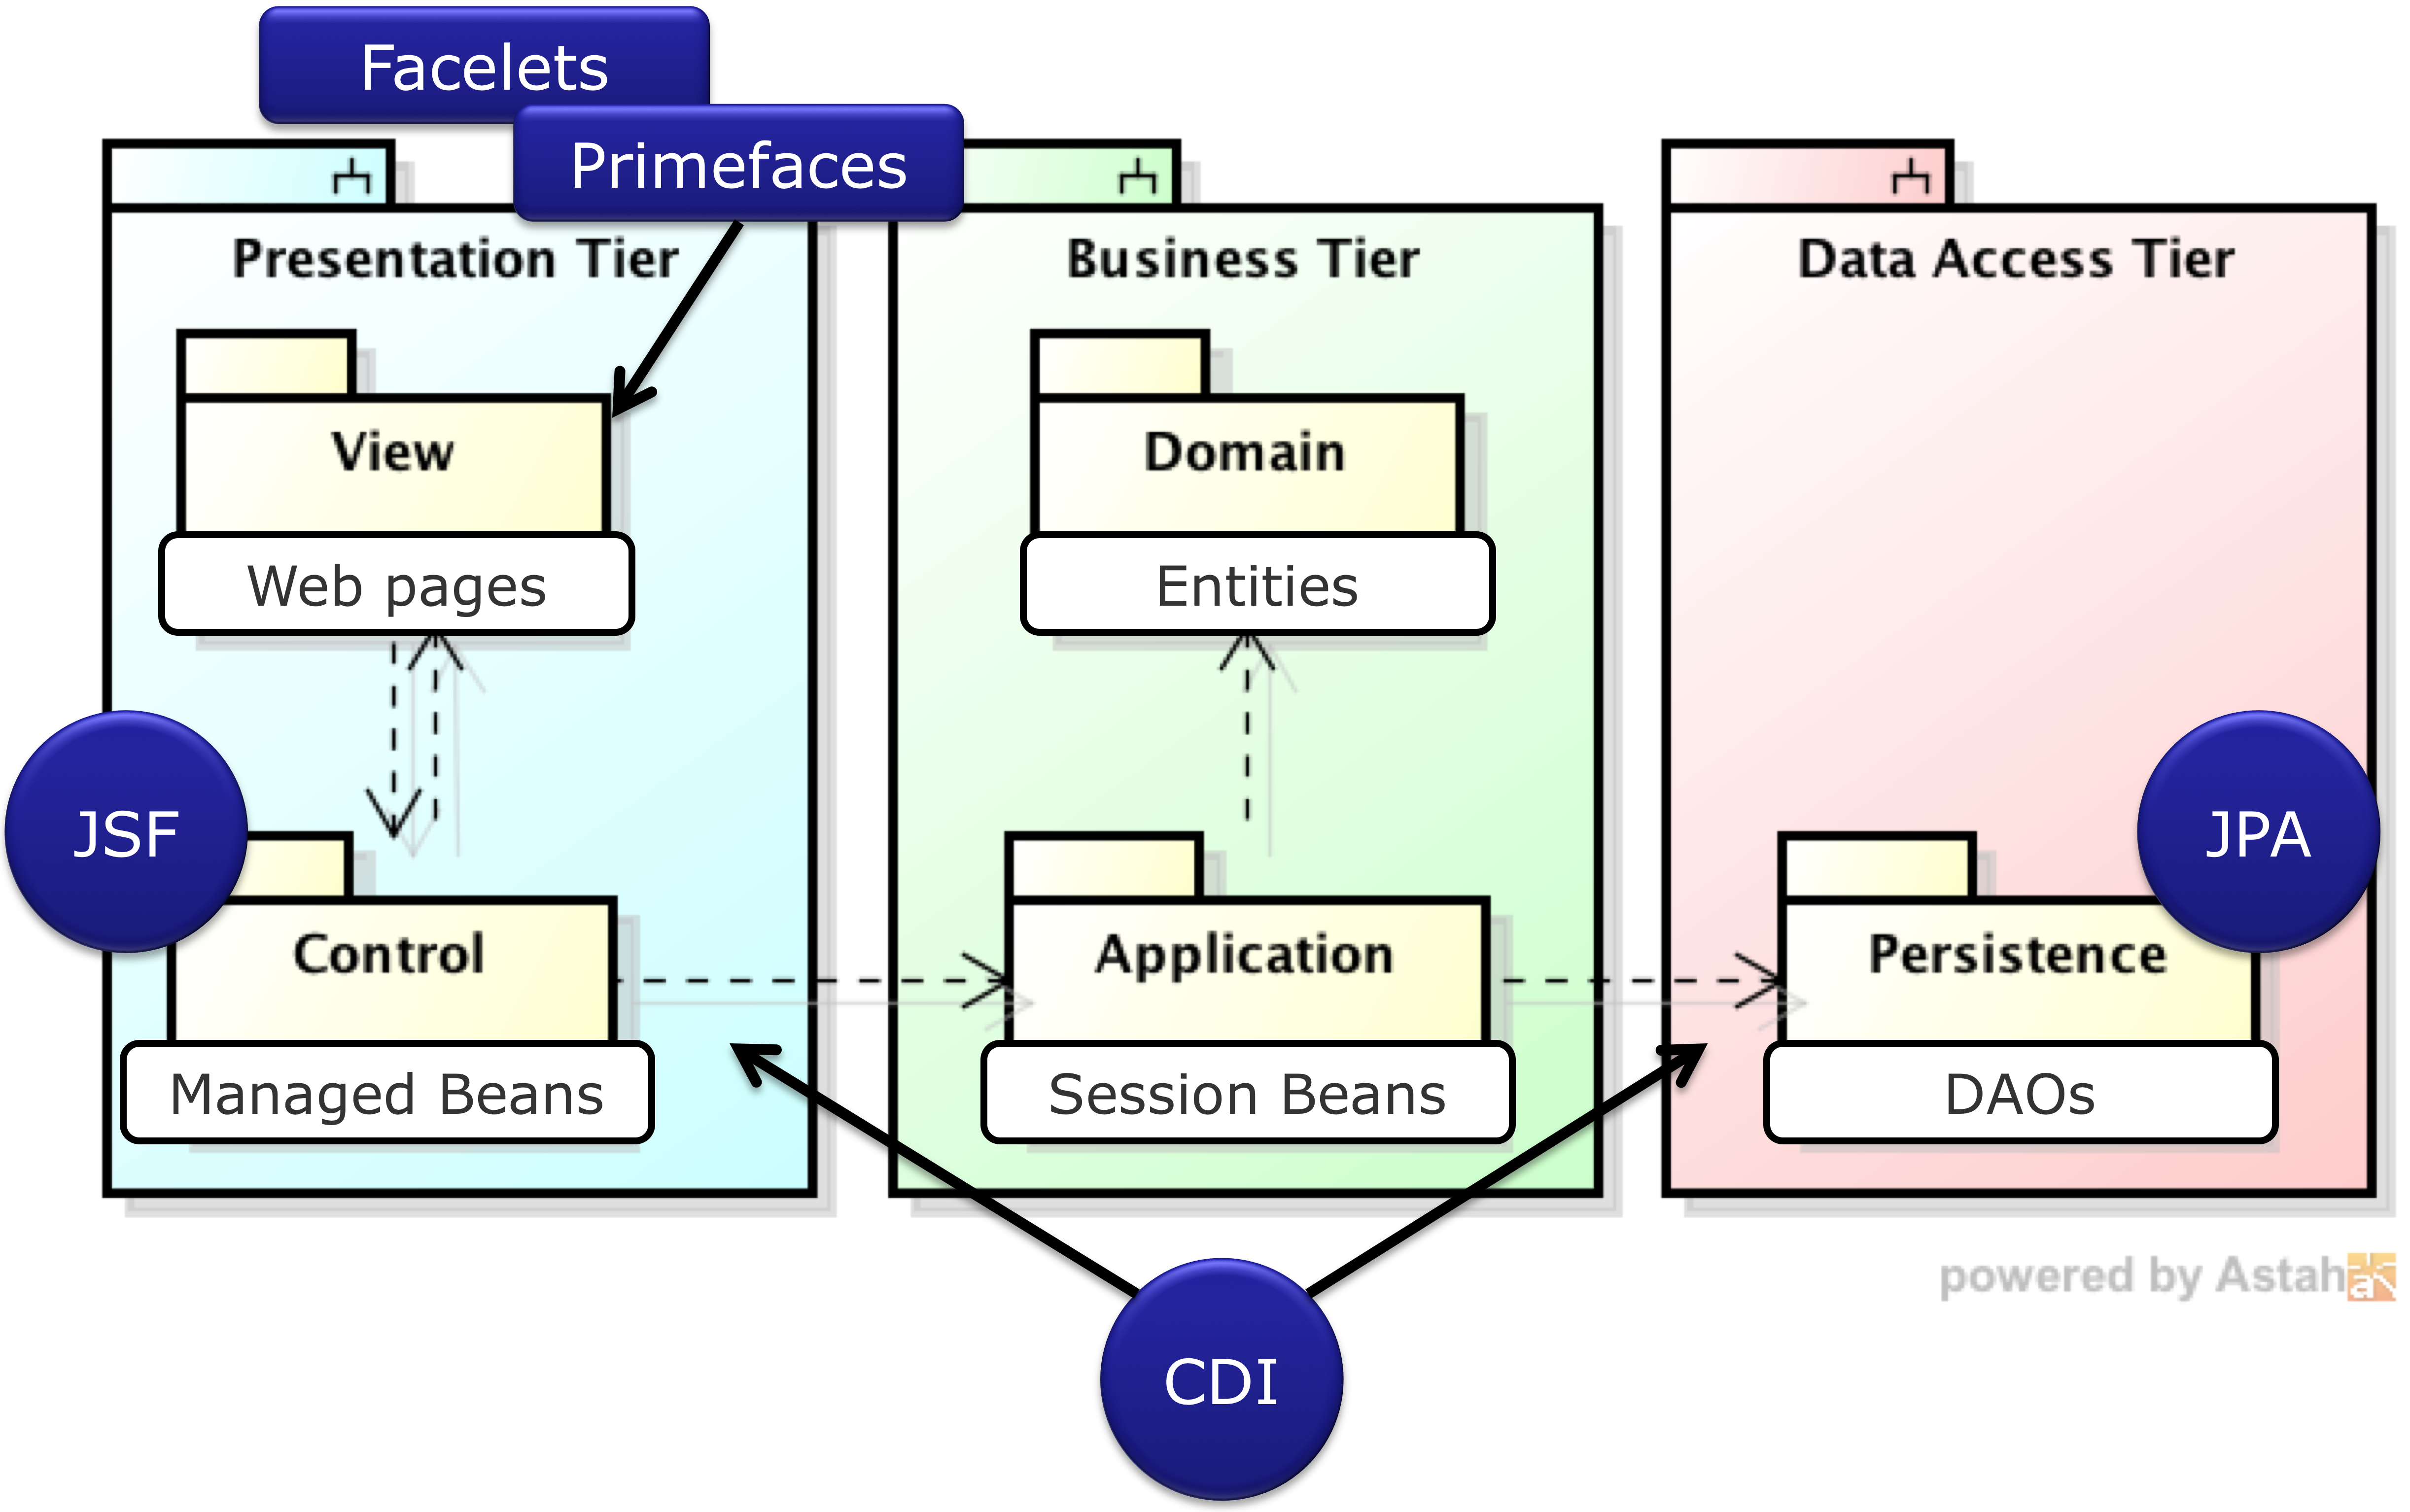
\includegraphics[width=0.7\textwidth]{figuras/figura-arquitetura-padrao.png}
	\caption{Arquitetura padrão proposta pelo FrameWeb.}
	\label{figura-arquitetura-padrao}
\end{figure}

Entretanto, como tal arquitetura não se mantém no padrão Django, que é composta de \textit{models}, \textit{views} e \textit{templates} com responsabilidades diferentes da dos elementos de mesmo nome na arquitetura Java EE. Portanto é necessario fazer aproximações para ambos os modelos dizerem a mesma coisa com palavras diferentes. Se adicionarmos uma camada de serviços entre os \textit{models} e \textit{views}, podemos obter uma arquitetura como a da Figura \ref{figura-arquitetura-adaptada}, que é bastante similar a \ref{figura-arquitetura-padrao}. Como Django usa \textit{Active Record} e não \textit{Data Access Objects}, a camada de acesso ao dado foi ignorada.

\begin{figure}[h]
	\centering
	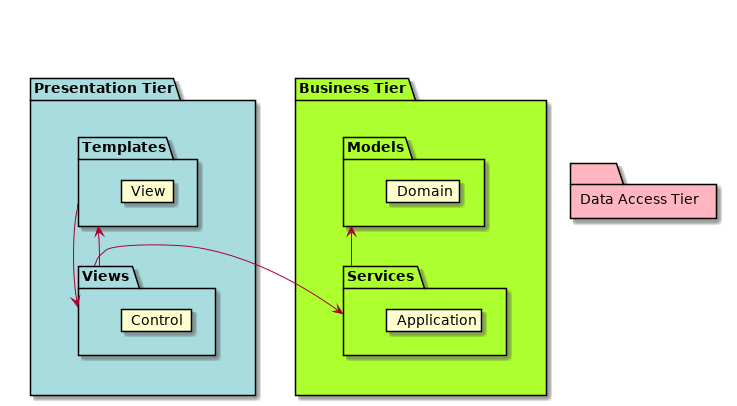
\includegraphics[width=0.7\textwidth, clip]{figuras/arquitetura.png}
	\caption{Arquitetura que busca aproximar o modelo do Django a do FrameWeb.}
	\label{figura-arquitetura-adaptada}
\end{figure}

Nas próximas seções, serão apresentados diagramas FrameWeb relativos a cada uma das camadas da arquitetura do sistema.

\section{Camada de Apresentação}
\label{sec-arquitetura-apresentacao}

% \vitor{Apresentar os modelos de navegação do FrameWeb.}

Como o sistema, ainda no estágio de projeto, ficou grande demais para ser representado em poucos modelos de navegação, cada diagrama desta seção não substitui o outro, mas representa por facetas complementares (não por partes) o sistema.

A Figura \ref{fig:nav0} traz as classes em seus respectivos pacotes que serão mencionados novamente no decorrer dos próximos parágrafos e figuras, mas tais classes serão mencionadas apenas pelo nome, estarão fora de seus respectivos pacotes e desprovidos de seus atributos e métodos, já que o intuito é melhorar a visualização dos dados através de uma organização mais flexível. Classes adicionais podem aparecer com nomes genéricos, indicando que são parte do \textit{framework} ou de alguma biblioteca; assume-se que sua existência e comportamento são conhecidos e, portanto, irrelevante modelar em detalhes. Como cada controlador está mapeado a uma rota e o método invocado é o verbo usado no protocolo HTTP, redirecionamentos de URL foram temporariamente representados no modelo como uma página que aciona o método \texttt{get} de algum controlador, levando a alguma outra página.

Os controladores do pacote \texttt{view} recebem até 3 parâmetros: uma instância de \texttt{HttpRequest}, um serviço e uma instância de alguma classe presente no modelo de entidades. A instância de \texttt{HttpRequest} contém, dentre várias coisas, o usuário atualmente autenticado no sistema e os parâmetros GET e POST, sendo fornecido pela \textit{framework}. O serviço é injetado por um decorador de uma biblioteca de injeção de dependências. A instância de alguma entidade é injetada por um transformador que, a partir de algum componente de URL nomeado que atua como identificador único, busca o objeto persistido e o insere como parâmetro do método. Todas as requisições são processadas em escopo de requisição, onde apenas alguns poucos dados (identificador de usuário logado, seleção de idioma e seleção de fuso-horário) são armazenados em cookies e variáveis de sessão.

Formulários (pacote \texttt{form}) representam apenas os campos do formulário, seu \textit{widget} de apresentação (para uso em templates), seus dados e seus validadores, podendo ser usado em classes que receberiam os estereótipos \textit{<<page>>}, \textit{<<controller>>} e \textit{<<service>>}, cada um com um diferente propósito: em páginas, exibiria os campos; em serviços, atua como validador e atualizador de entidades; em controladores, facilita o encapsulamento em poucas linhas dos dados de formulário (fornecidos pela instância de \texttt{HttpRequest}) e, caso a validação falhe, a exibição dos erros de validação na mesma página em que o formulário foi editado.

\begin{figure}
	\centering
	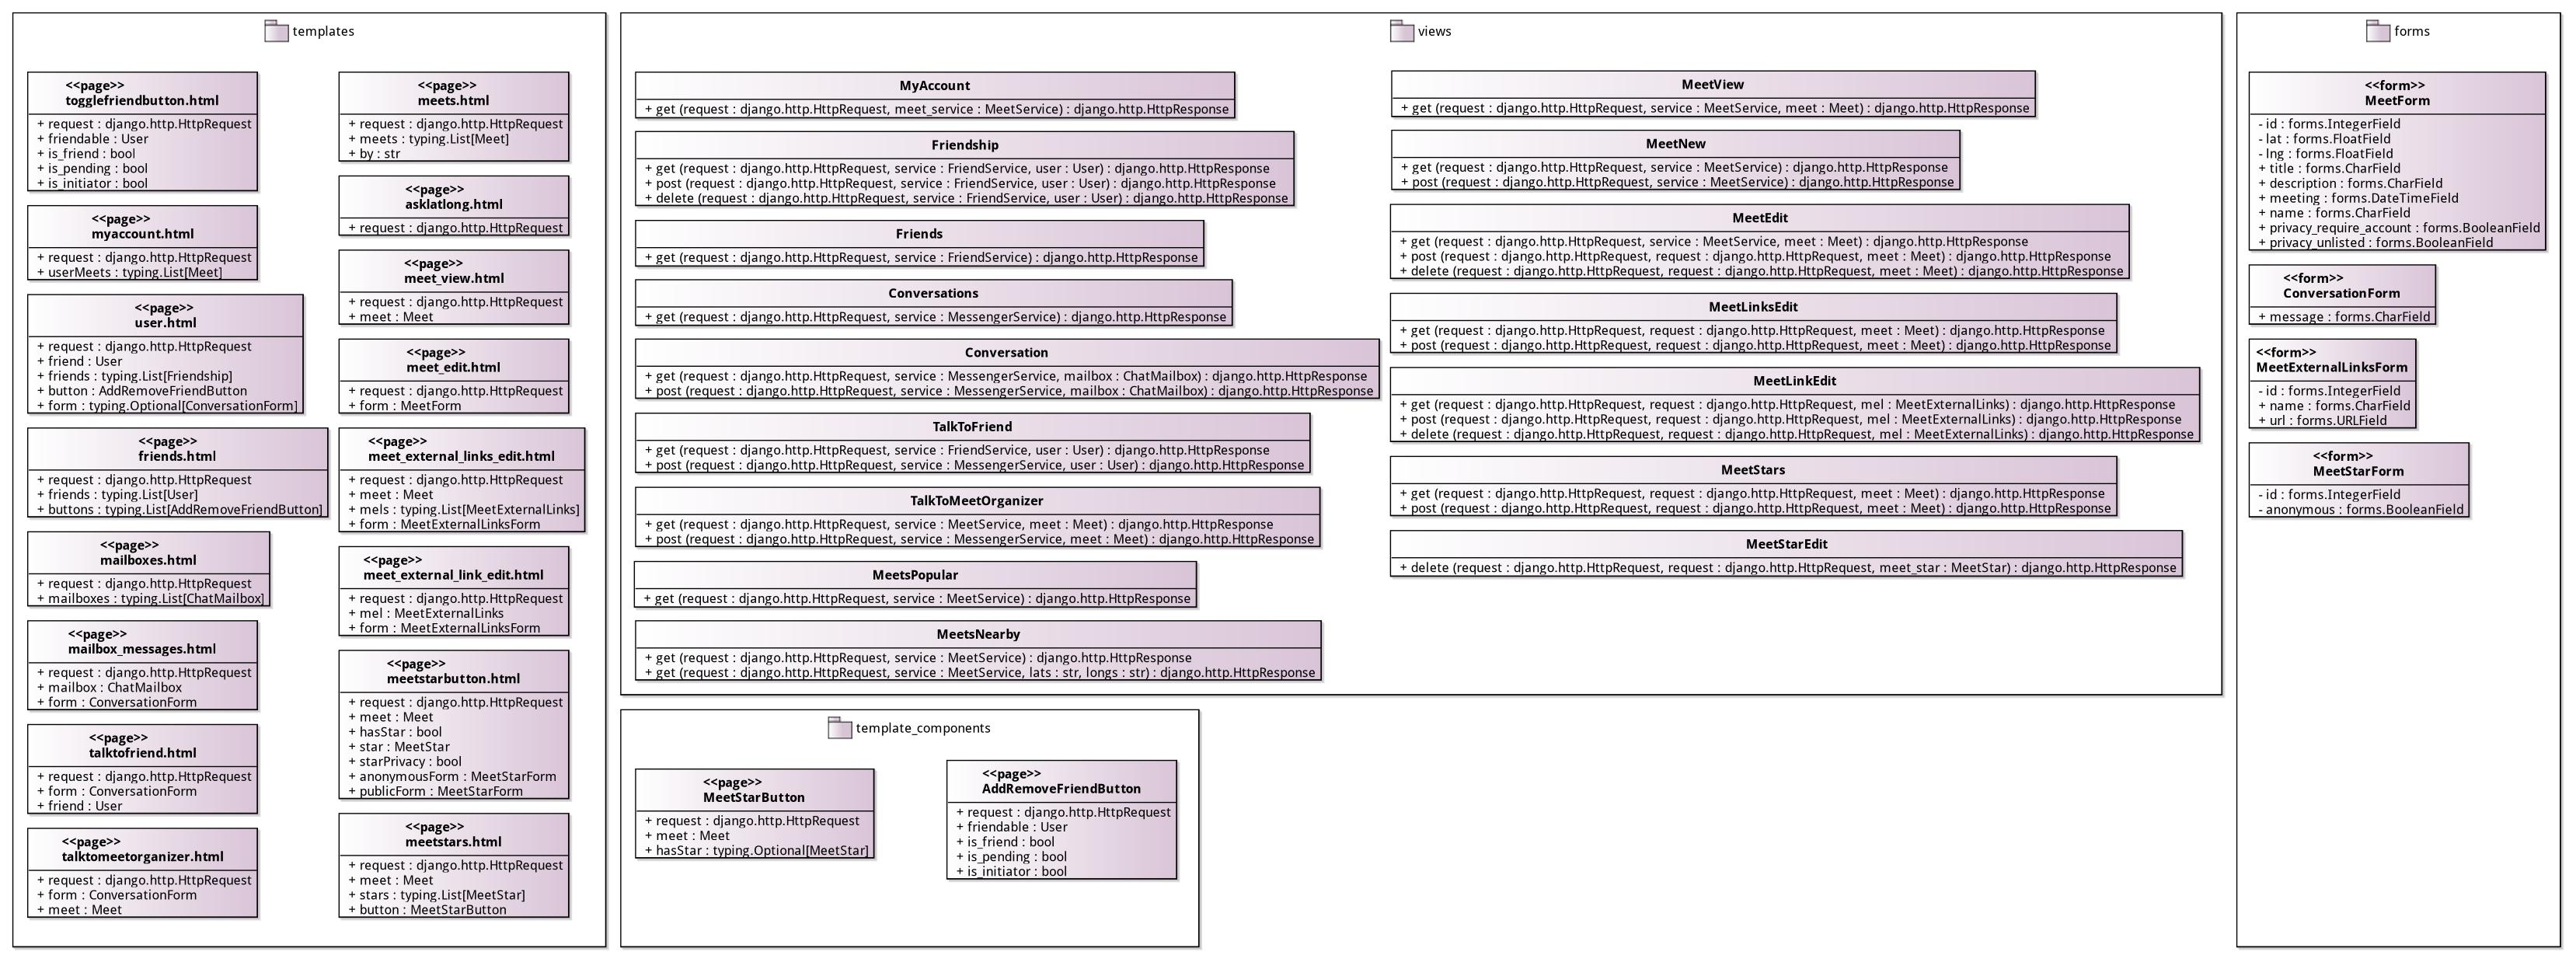
\includegraphics[width=0.8\paperheight, angle=270]{figuras/FrameWebNavigationModel.jpg}
	\caption{Modelo de Navegação do \imprimirtitulo{} -- Apenas classes}
	\label{fig:nav0}
\end{figure}

A Figura \ref{fig:nav1} mostra a navegação de uma página acessível publicamente para uma página que é acessível somente a usuários, mostrando a possibilidade de ser redirecionado para uma tela de login, que, depois de logado, redireciona de volta à página originalmente solicitada. São controladores acessíveis apenas a usuários logados:
\begin{itemize}
  \item \texttt{MyAccount}
  \item \texttt{Friendship} (apenas métodos \texttt{post} e \texttt{delete})
  \item \texttt{Friends}
  \item \texttt{Conversations}
  \item \texttt{Conversation}
  \item \texttt{TalkToFriend}
  \item \texttt{TalkToMeetOrganizer}
  \item \texttt{MeetNew}
  \item \texttt{MeetEdit}
  \item \texttt{MeetLinksEdit}
  \item \texttt{MeetLinkEdit}
  \item \texttt{MeetStars} (apenas método \texttt{post})
  \item \texttt{MeetStarEdit}
\end{itemize}

\begin{figure}[H]
	\centering
	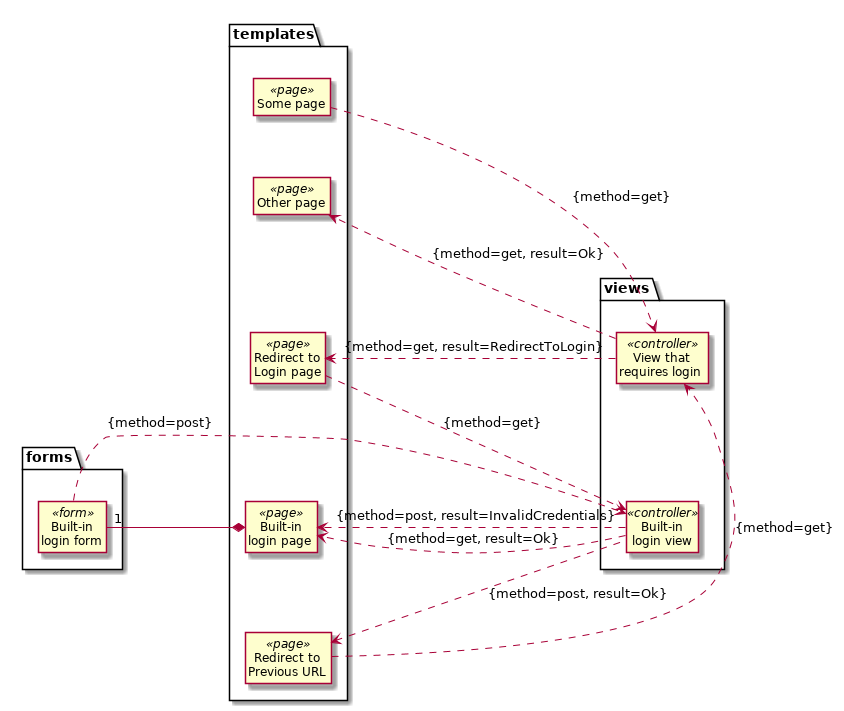
\includegraphics[scale=0.5]{figuras/navigation-extra.png}
	\caption{Modelo de Navegação do \imprimirtitulo{} -- Login para acessar algum recurso}
	\label{fig:nav1}
\end{figure}

A Figura \ref{fig:shortcut1:0} mostra a navegação entre duas páginas que possuem autorreferência, e observa-se que o modelo acaba um tanto poluído. Tomando a liberdade para estender o modelo padrão padrão do FrameWeb, adiciona-se o estereótipo <<controls>> vinculando uma página a um controlador (Figura \ref{fig:shortcut1:1}), na qual aquele controlador será controlado apenas por aquele controlador para todos os métodos a menos que explicitamente mencionado o contrário, e setas contíguas no modelo de navegação representam uma requisição ao método \texttt{get} do controlador seguido de uma resposta bem-sucedida à página com estereótipo <<controlledpage>> (Figura \ref{fig:shortcut1:2}); considera-se a seta de linha contínua um comportamento explícito. Caso o controlador implemente outros métodos, a Figura \ref{fig:shortcut1:3} ilustra o comportamento padrão esperado. Outro atalho que será introduzido é a seta pontilhada com \texttt{result=redirect} de controlador para controlador, que abstrai uma página de redirecionamento, acionando o método \texttt{get} do controlador que recebe a requisição (Figura \ref{fig:shortcut2}). Ainda outra abstração é o método ``\texttt{*}'', que significa ``qualquer método não explicitamente modelado''.

\begin{figure}[H]
	\centering
	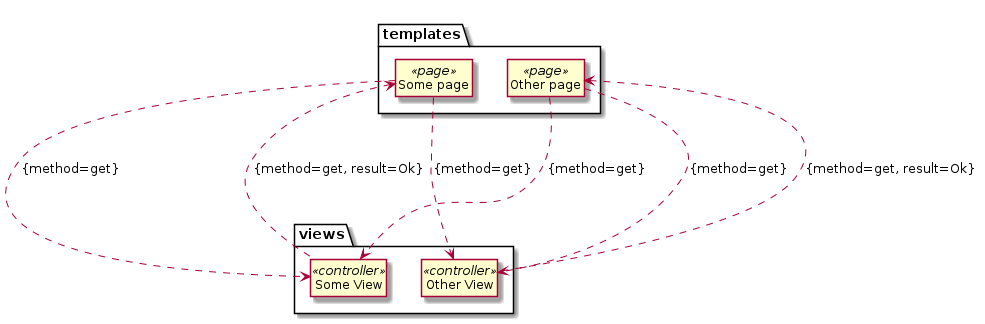
\includegraphics[scale=0.4]{figuras/navigation-shortcut1.png}
	\caption{Modelo que busca justificar a necessidade de estender a linguagem do FrameWeb}
	\label{fig:shortcut1:0}
\end{figure}
\begin{figure}[H]
	\centering
	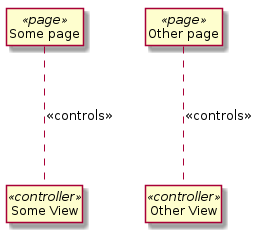
\includegraphics[scale=0.5]{figuras/navigation-shortcut1_2.png}
	\caption{Atalho proposto para modelo de Navegação do \imprimirtitulo{} -- Modelo que propõe um atalho, introduzindo o estereótipo <<controls>>}
	\label{fig:shortcut1:1}
\end{figure}
\begin{figure}[H]
	\centering
	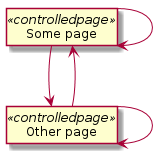
\includegraphics[scale=0.5]{figuras/navigation-shortcut1_3.png}
	\caption{Atalho proposto para modelo de Navegação do \imprimirtitulo{} -- Modelo que porpõe um atalho, introduzindo a seta cheia e o estereótipo <<controlledpage>>}
	\label{fig:shortcut1:2}
\end{figure}
\begin{figure}[H]
	\centering
	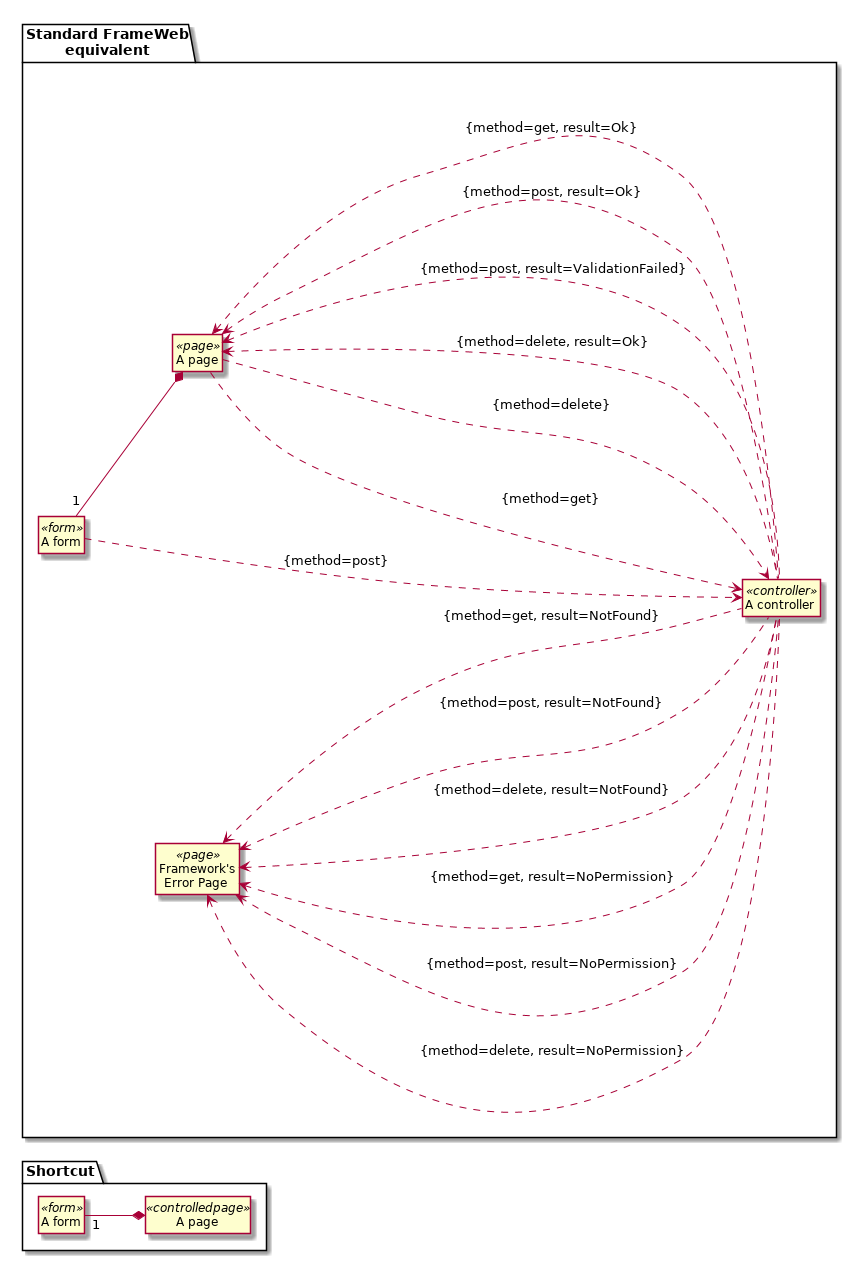
\includegraphics[scale=0.5]{figuras/navigation-shortcut1_4.png}
	\caption{Atalho proposto para modelo de Navegação do \imprimirtitulo{} -- Modelo que porpõe um atalho, explicitando todo o ciclo de vida implícito de um <<controlledpage>> com formulário}
	\label{fig:shortcut1:3}
\end{figure}
\begin{figure}[H]
	\centering
	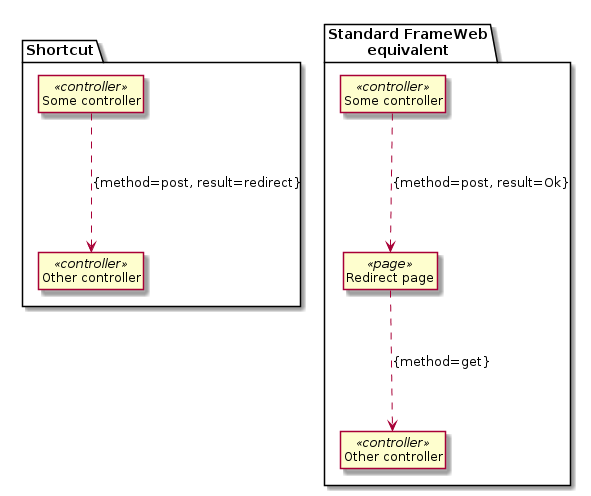
\includegraphics[scale=0.5]{figuras/navigation-shortcut2.png}
	\caption{Atalho proposto para modelo de Navegação do \imprimirtitulo{} -- Modelo que porpõe um atalho para ligar o redirecionamento de um controlador diretamente no método \textit{get} em outro controlador}
	\label{fig:shortcut2}
\end{figure}

Logo, podemos fazer uso de todos os atalhos apresentados acima apresentar as associações na Figura \ref{fig:shortcut1:res1} e montar o modelo de navegação na Figura \ref{fig:shortcut1:res2}.

\begin{figure}[H]
	\centering
	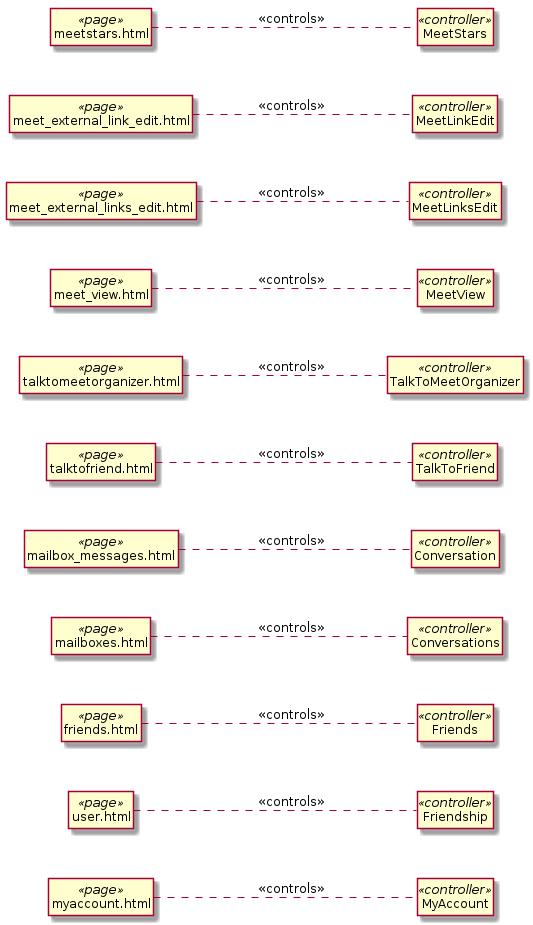
\includegraphics[scale=0.5]{figuras/navigation-shortcut1_res1.png}
	\caption{Modelo de Navegação do \imprimirtitulo{} com atalhos -- Controladores das páginas}
	\label{fig:shortcut1:res1}
\end{figure}

\begin{figure}[H]
	\centering
	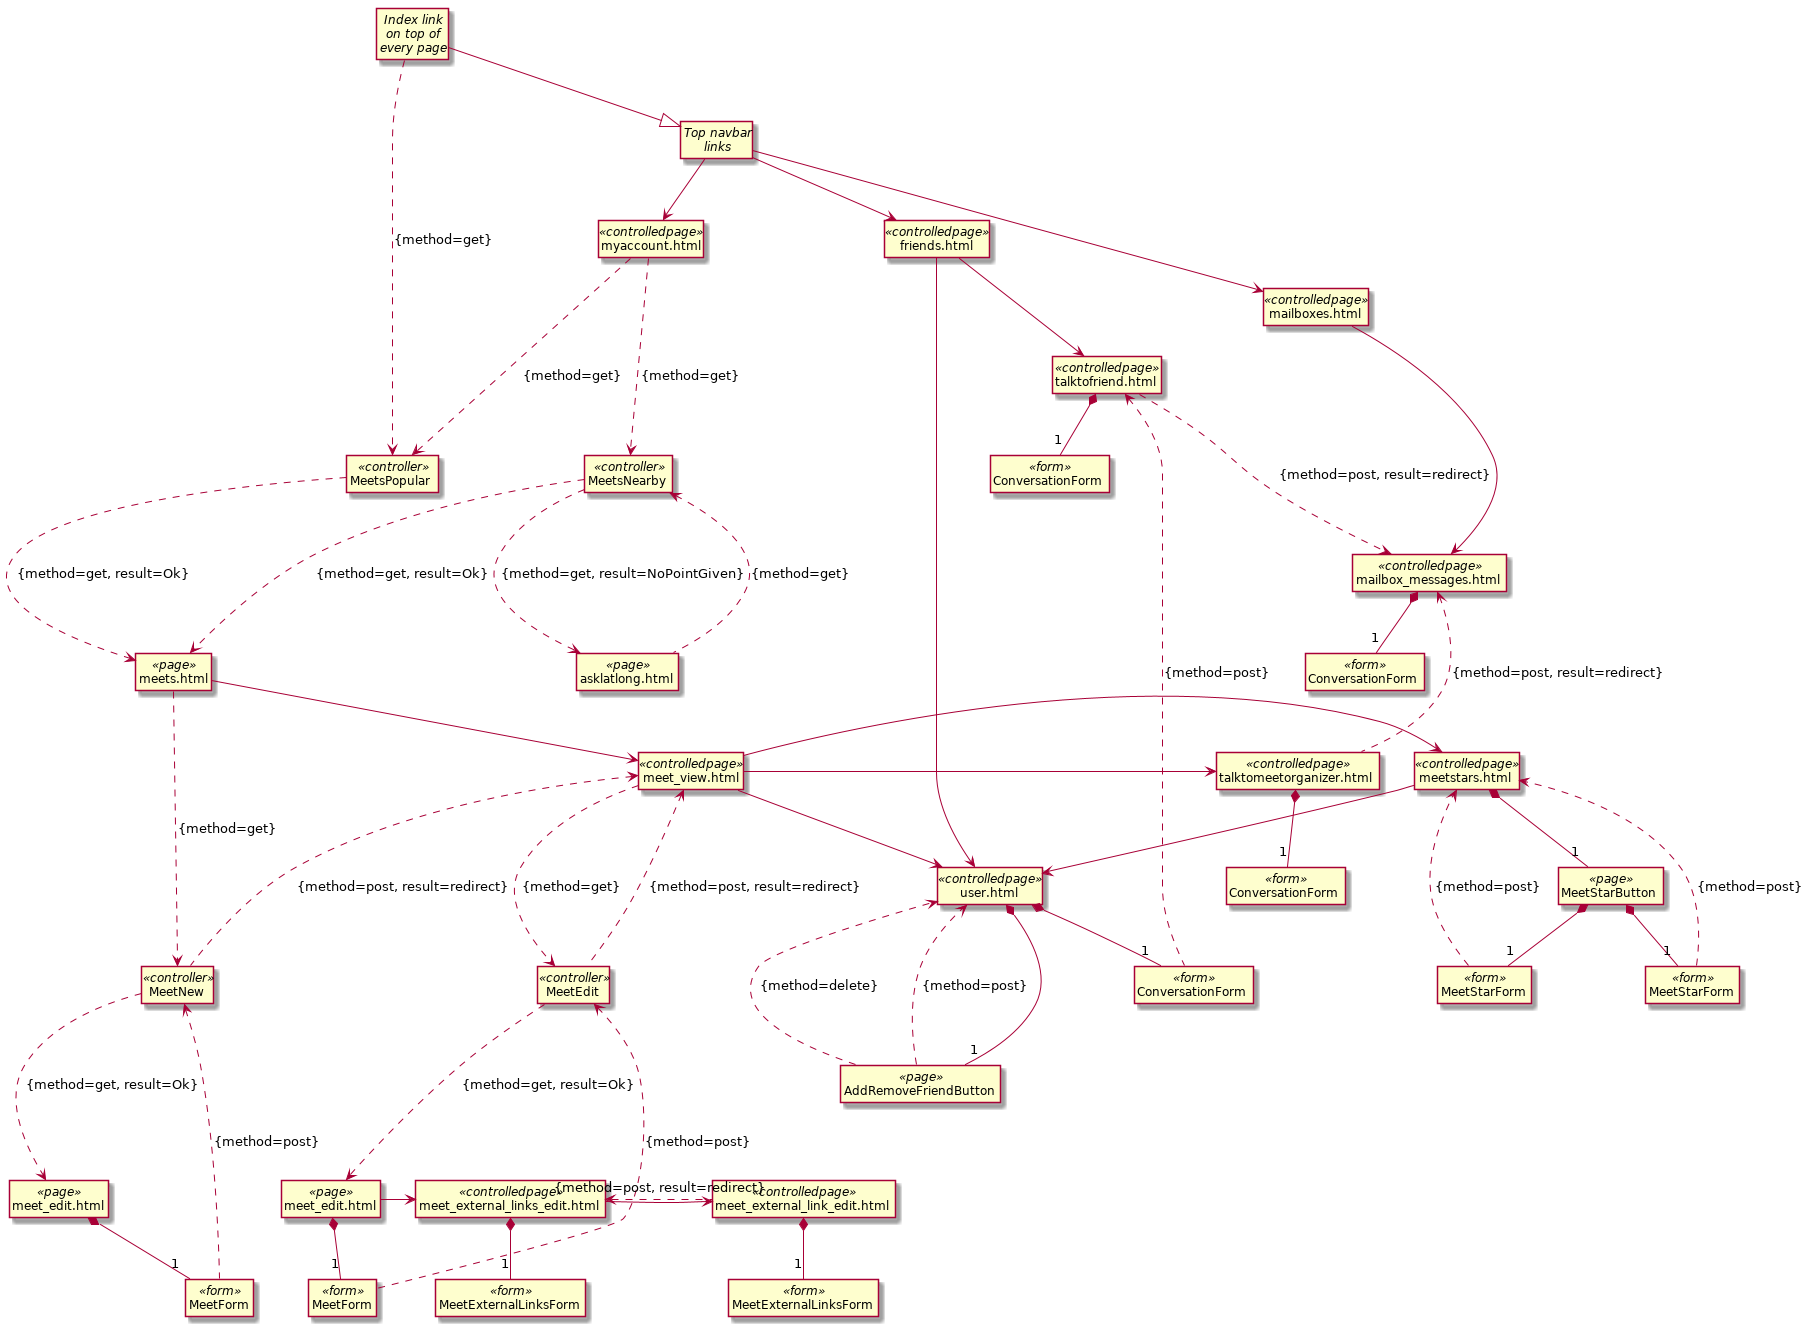
\includegraphics[scale=0.25]{figuras/navigation-shortcut1_res2.png}
	\caption{Modelo de Navegação do \imprimirtitulo{} com atalhos -- Navegação entre as páginas}
	\label{fig:shortcut1:res2}
\end{figure}


% \begin{figure}[H]
% 	\centering
% 	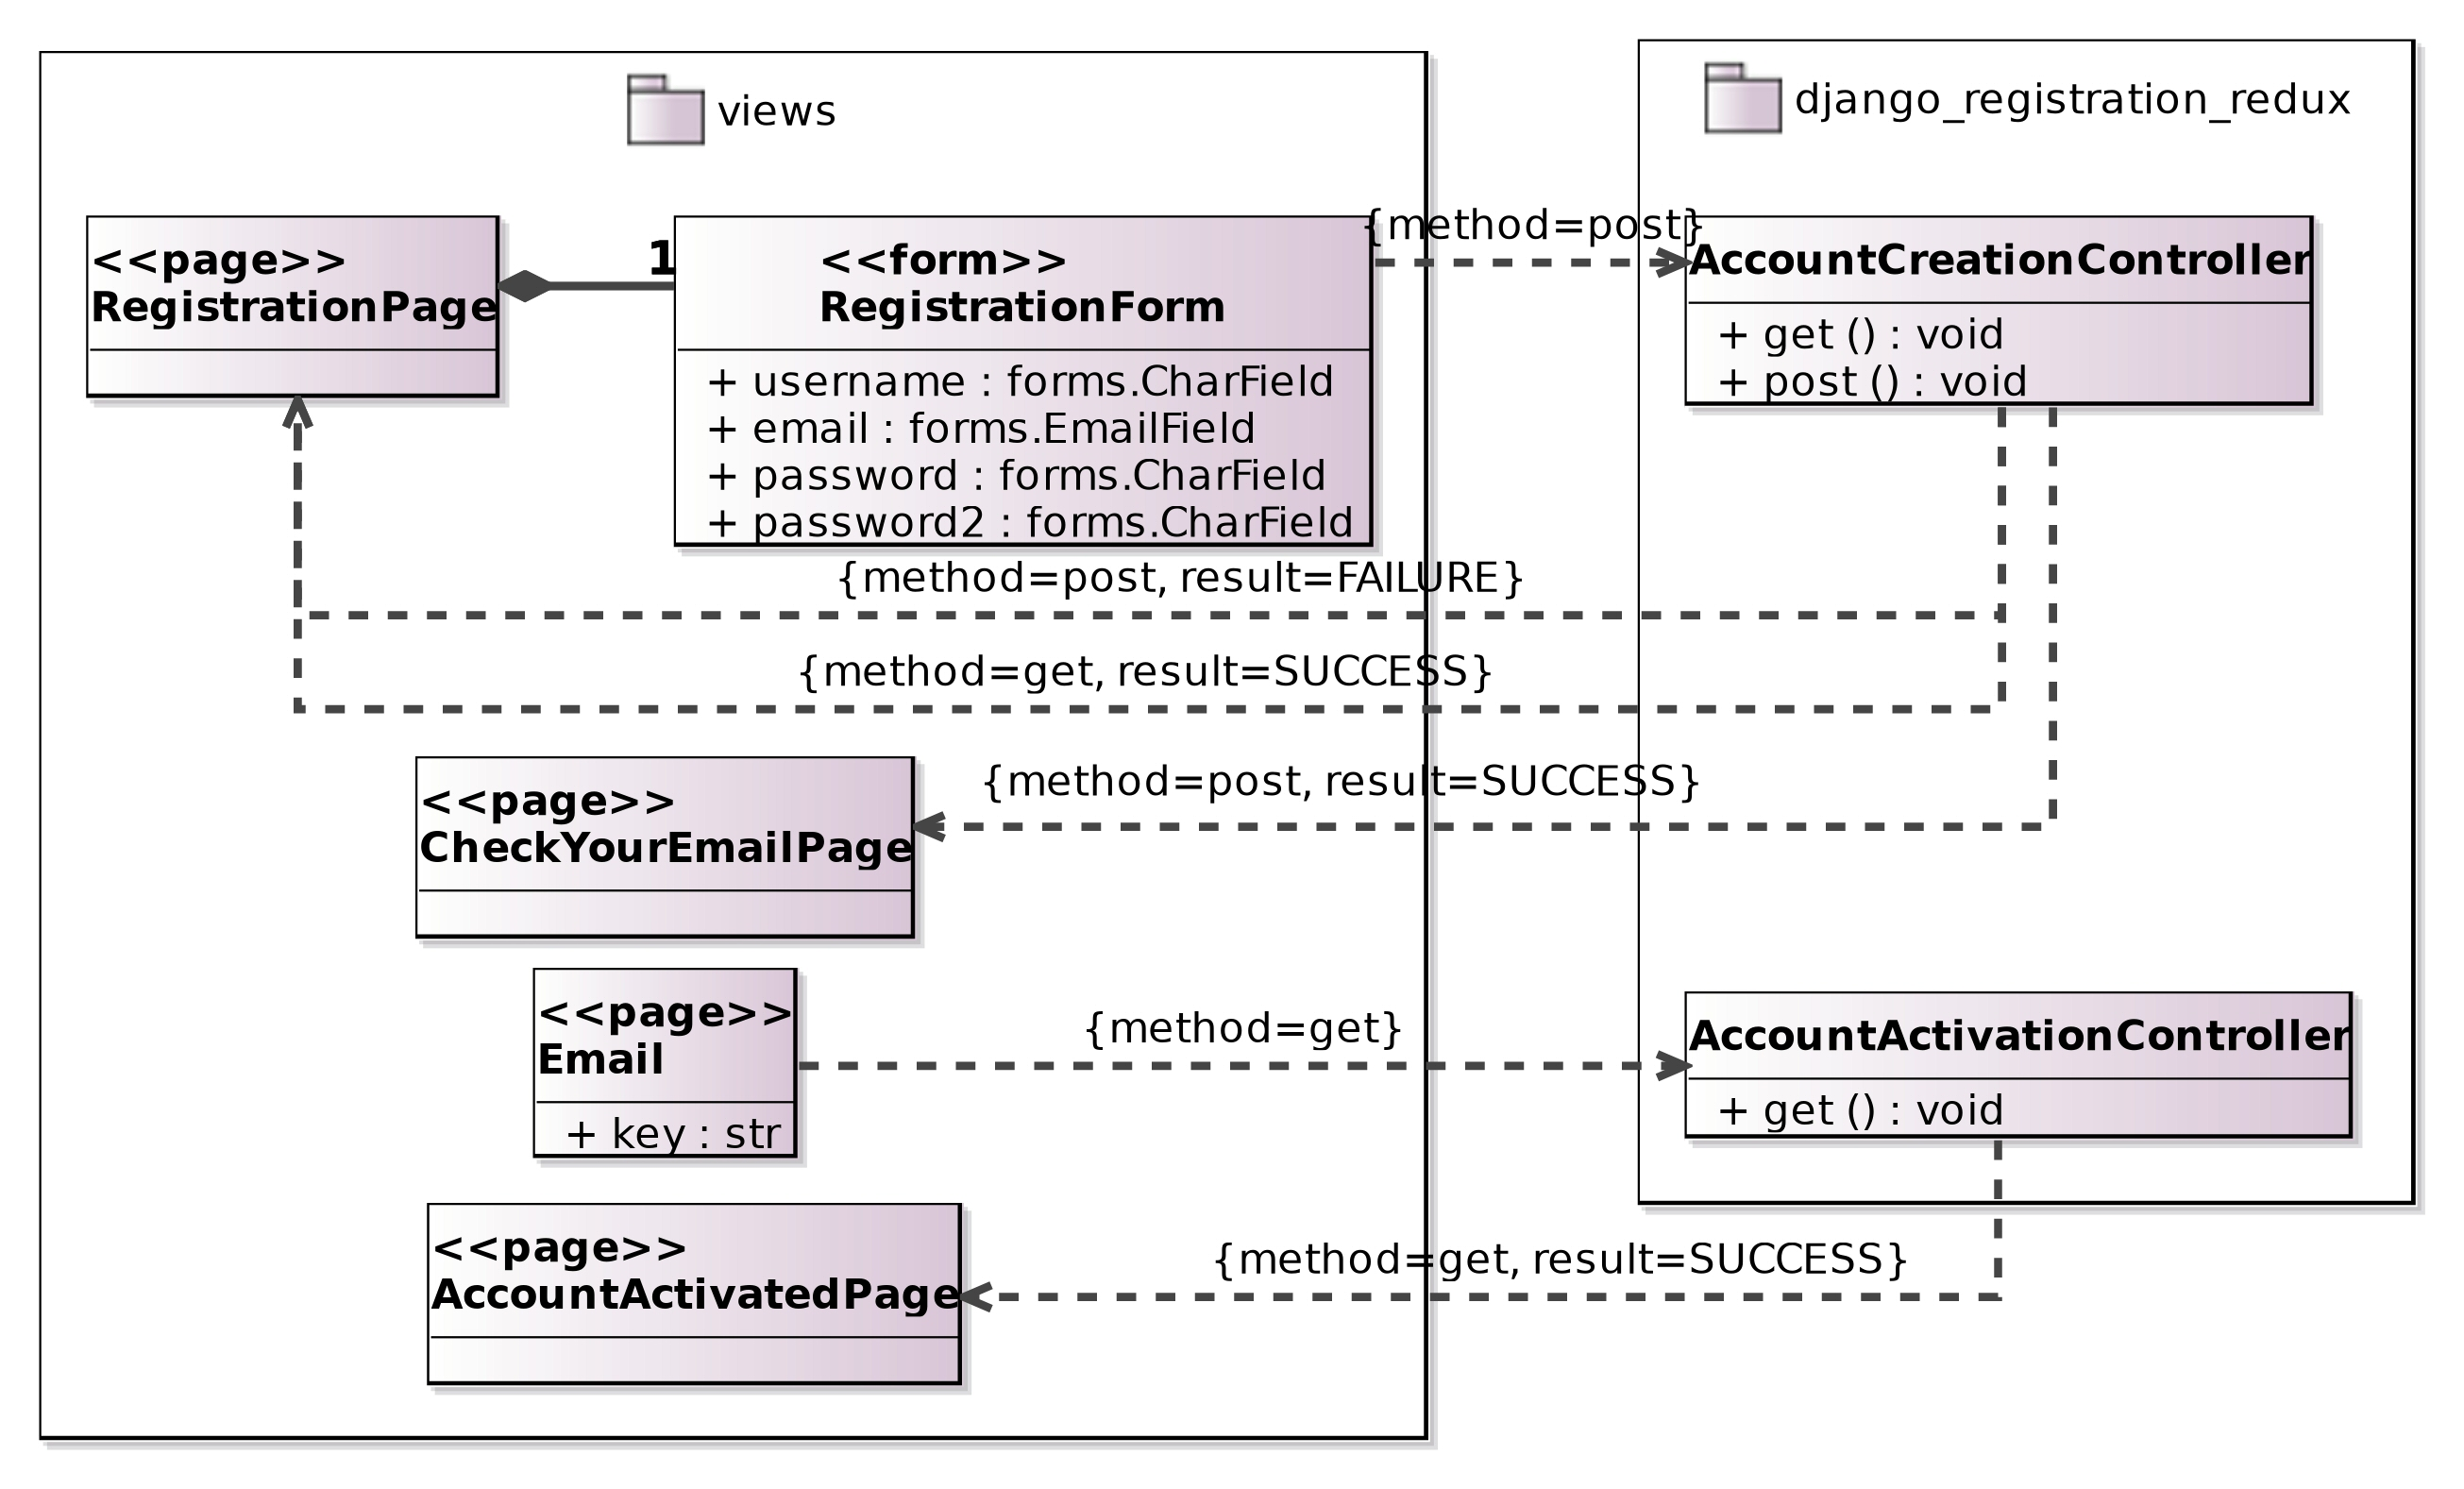
\includegraphics[scale=0.15]{figuras/FrameWebNavigationModel2.jpg}
% 	\caption{Modelo de Navegação do \imprimirtitulo{} -- Criar conta}
% 	\label{fig:nav2}
% \end{figure}
%
% \begin{figure}[H]
% 	\centering
% 	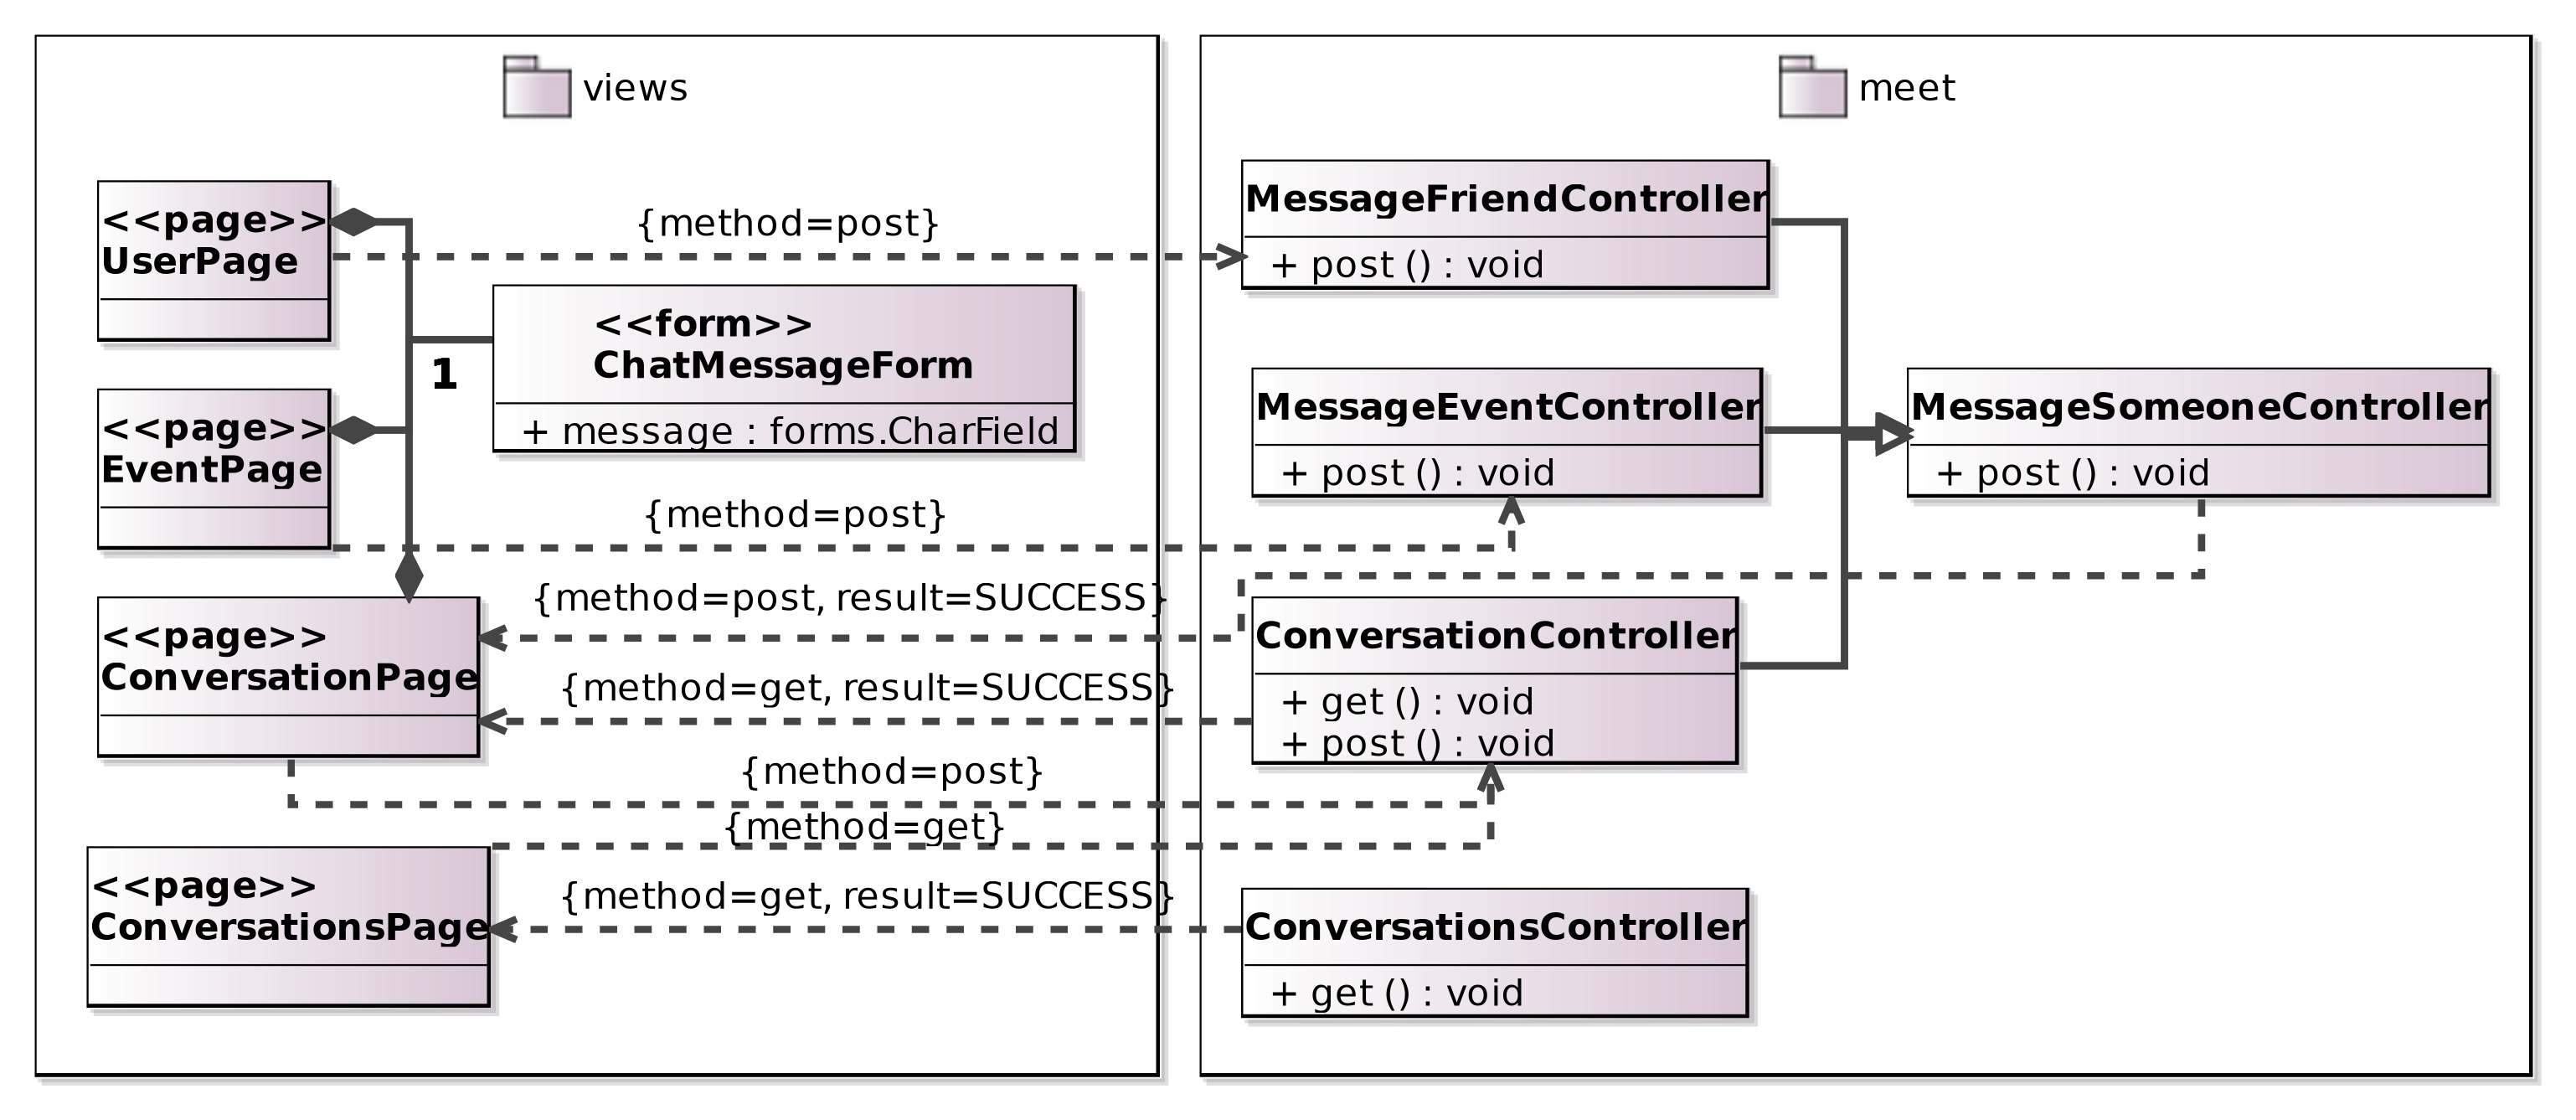
\includegraphics[scale=0.15]{figuras/FrameWebNavigationModel3.jpg}
% 	\caption{Modelo de Navegação do \imprimirtitulo{} -- Iniciar e continuar conversas}
% 	\label{fig:nav3}
% \end{figure}
%
% \begin{figure}[H]
% 	\centering
% 	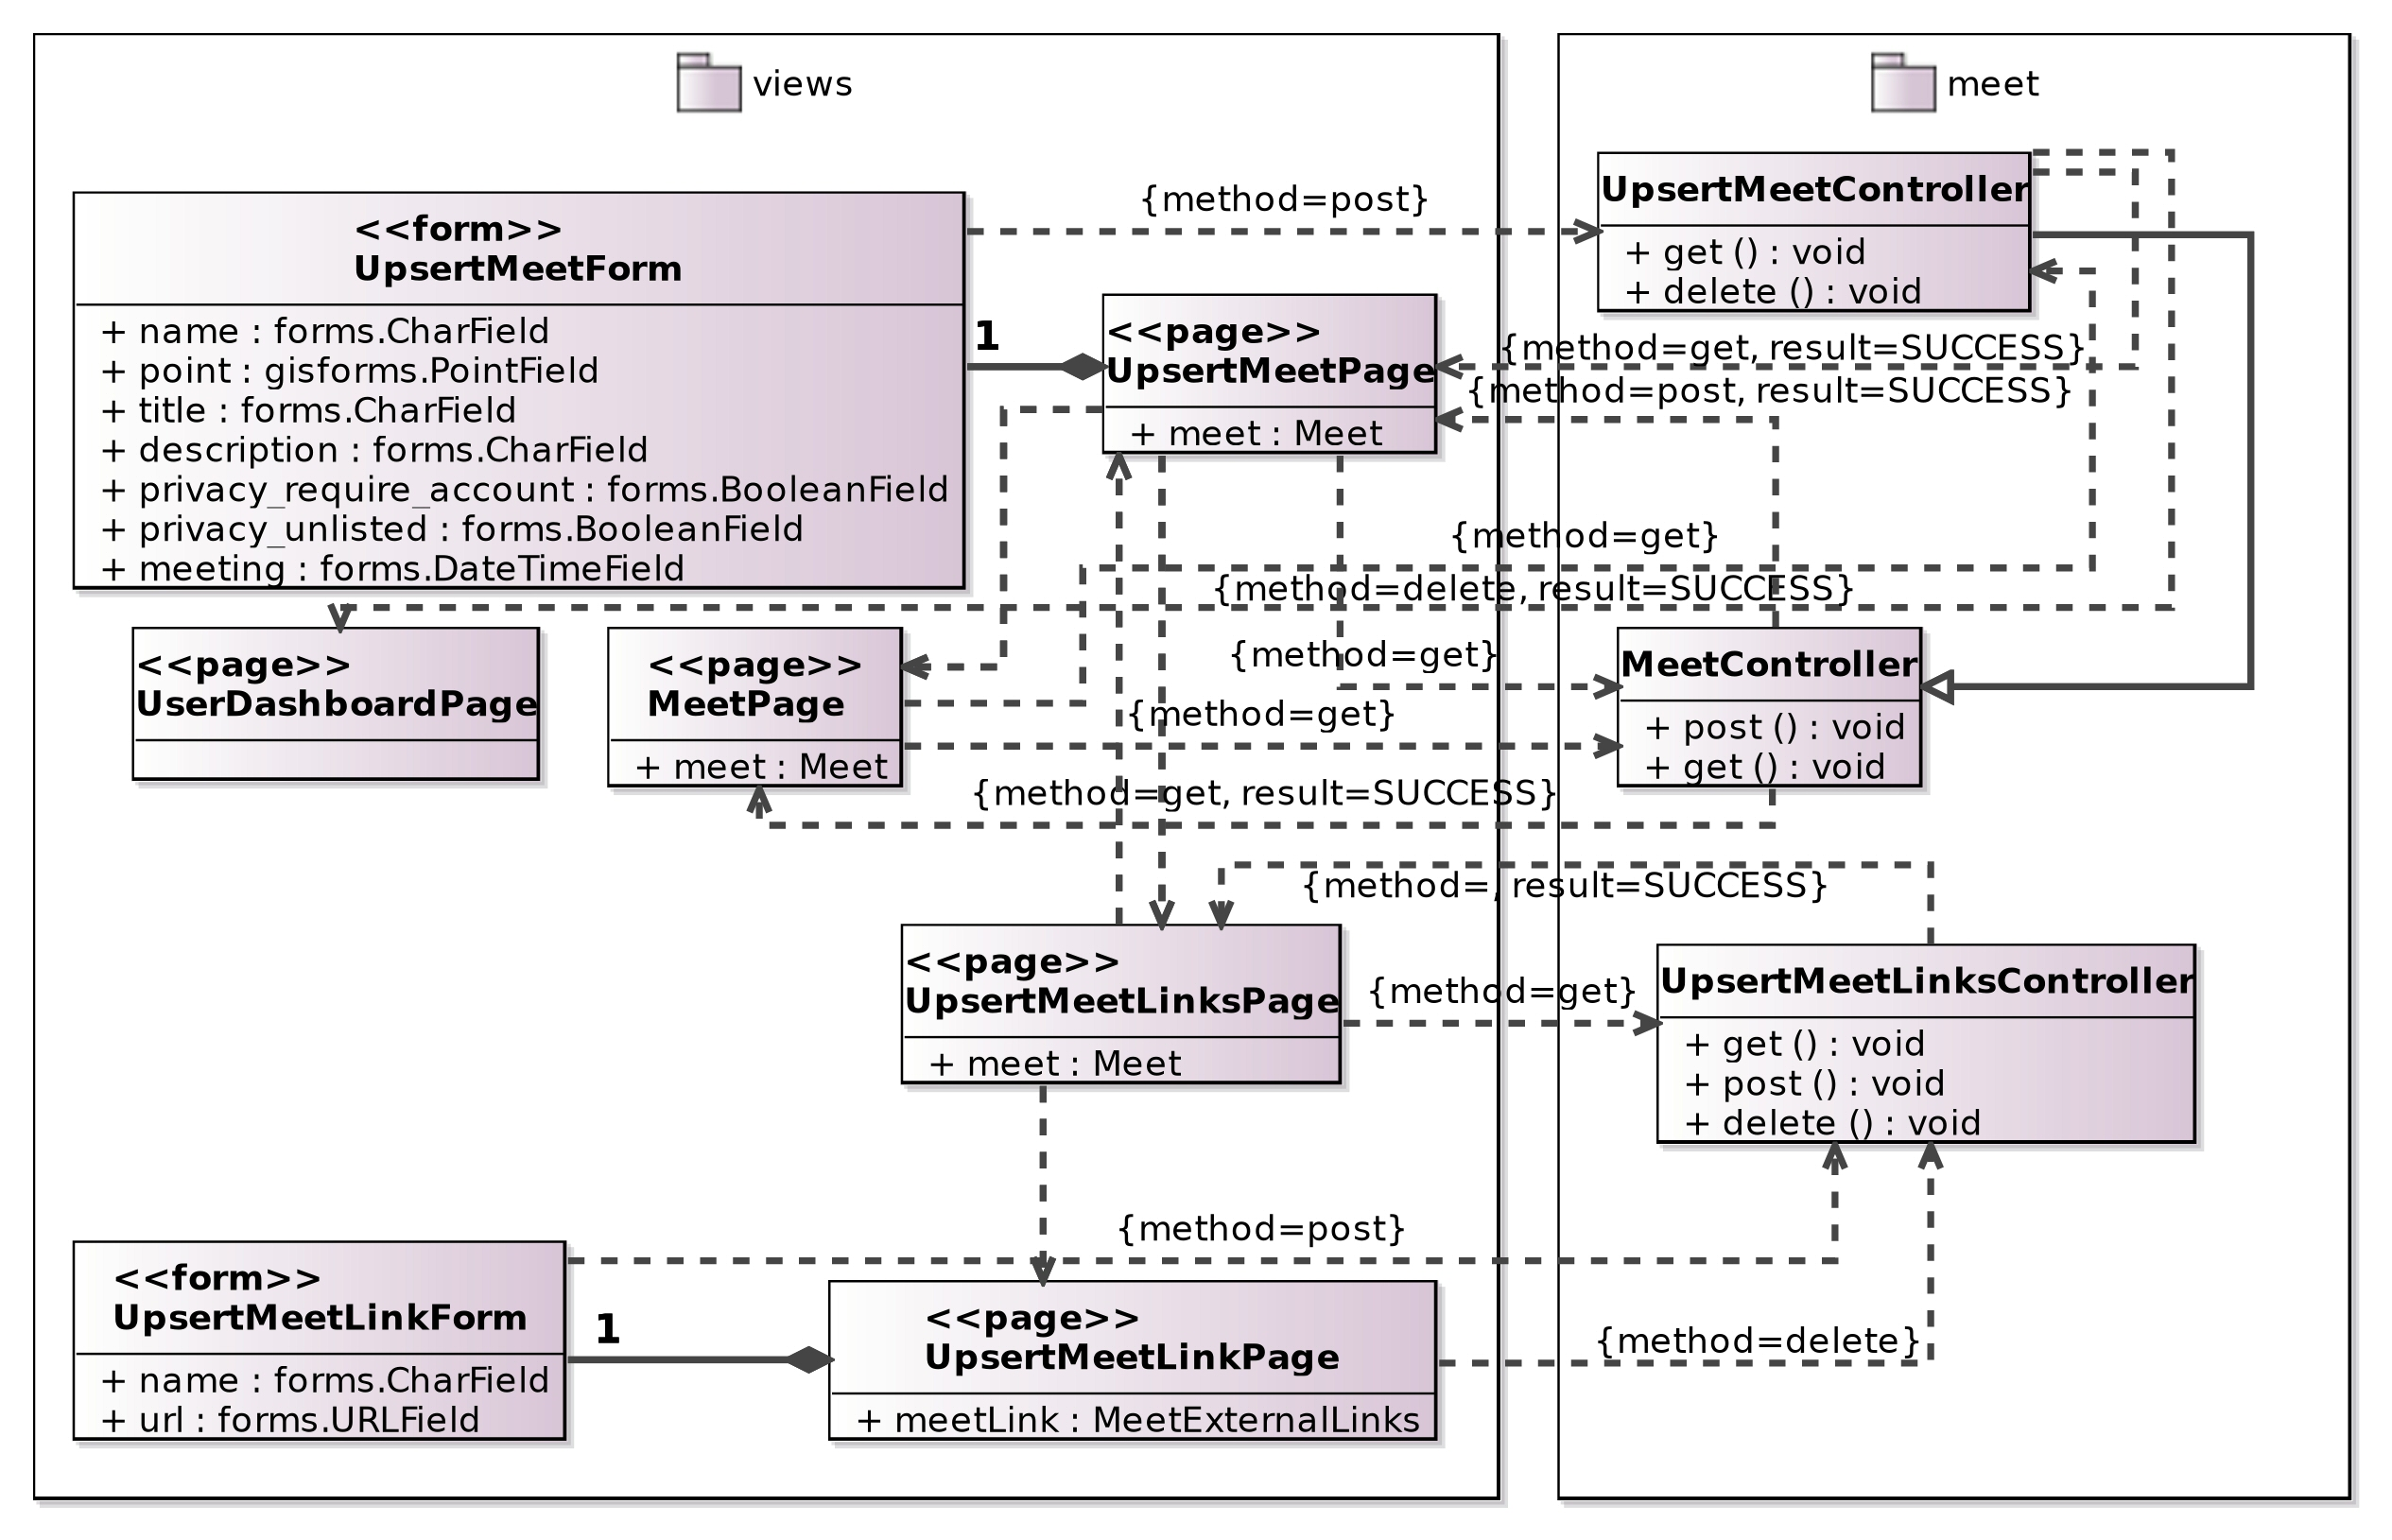
\includegraphics[scale=0.15]{figuras/FrameWebNavigationModel4.jpg}
% 	\caption{Modelo de Navegação do \imprimirtitulo{} -- Gerenciar encontros}
% 	\label{fig:nav4}
% \end{figure}
%
% \begin{figure}[H]
% 	\centering
% 	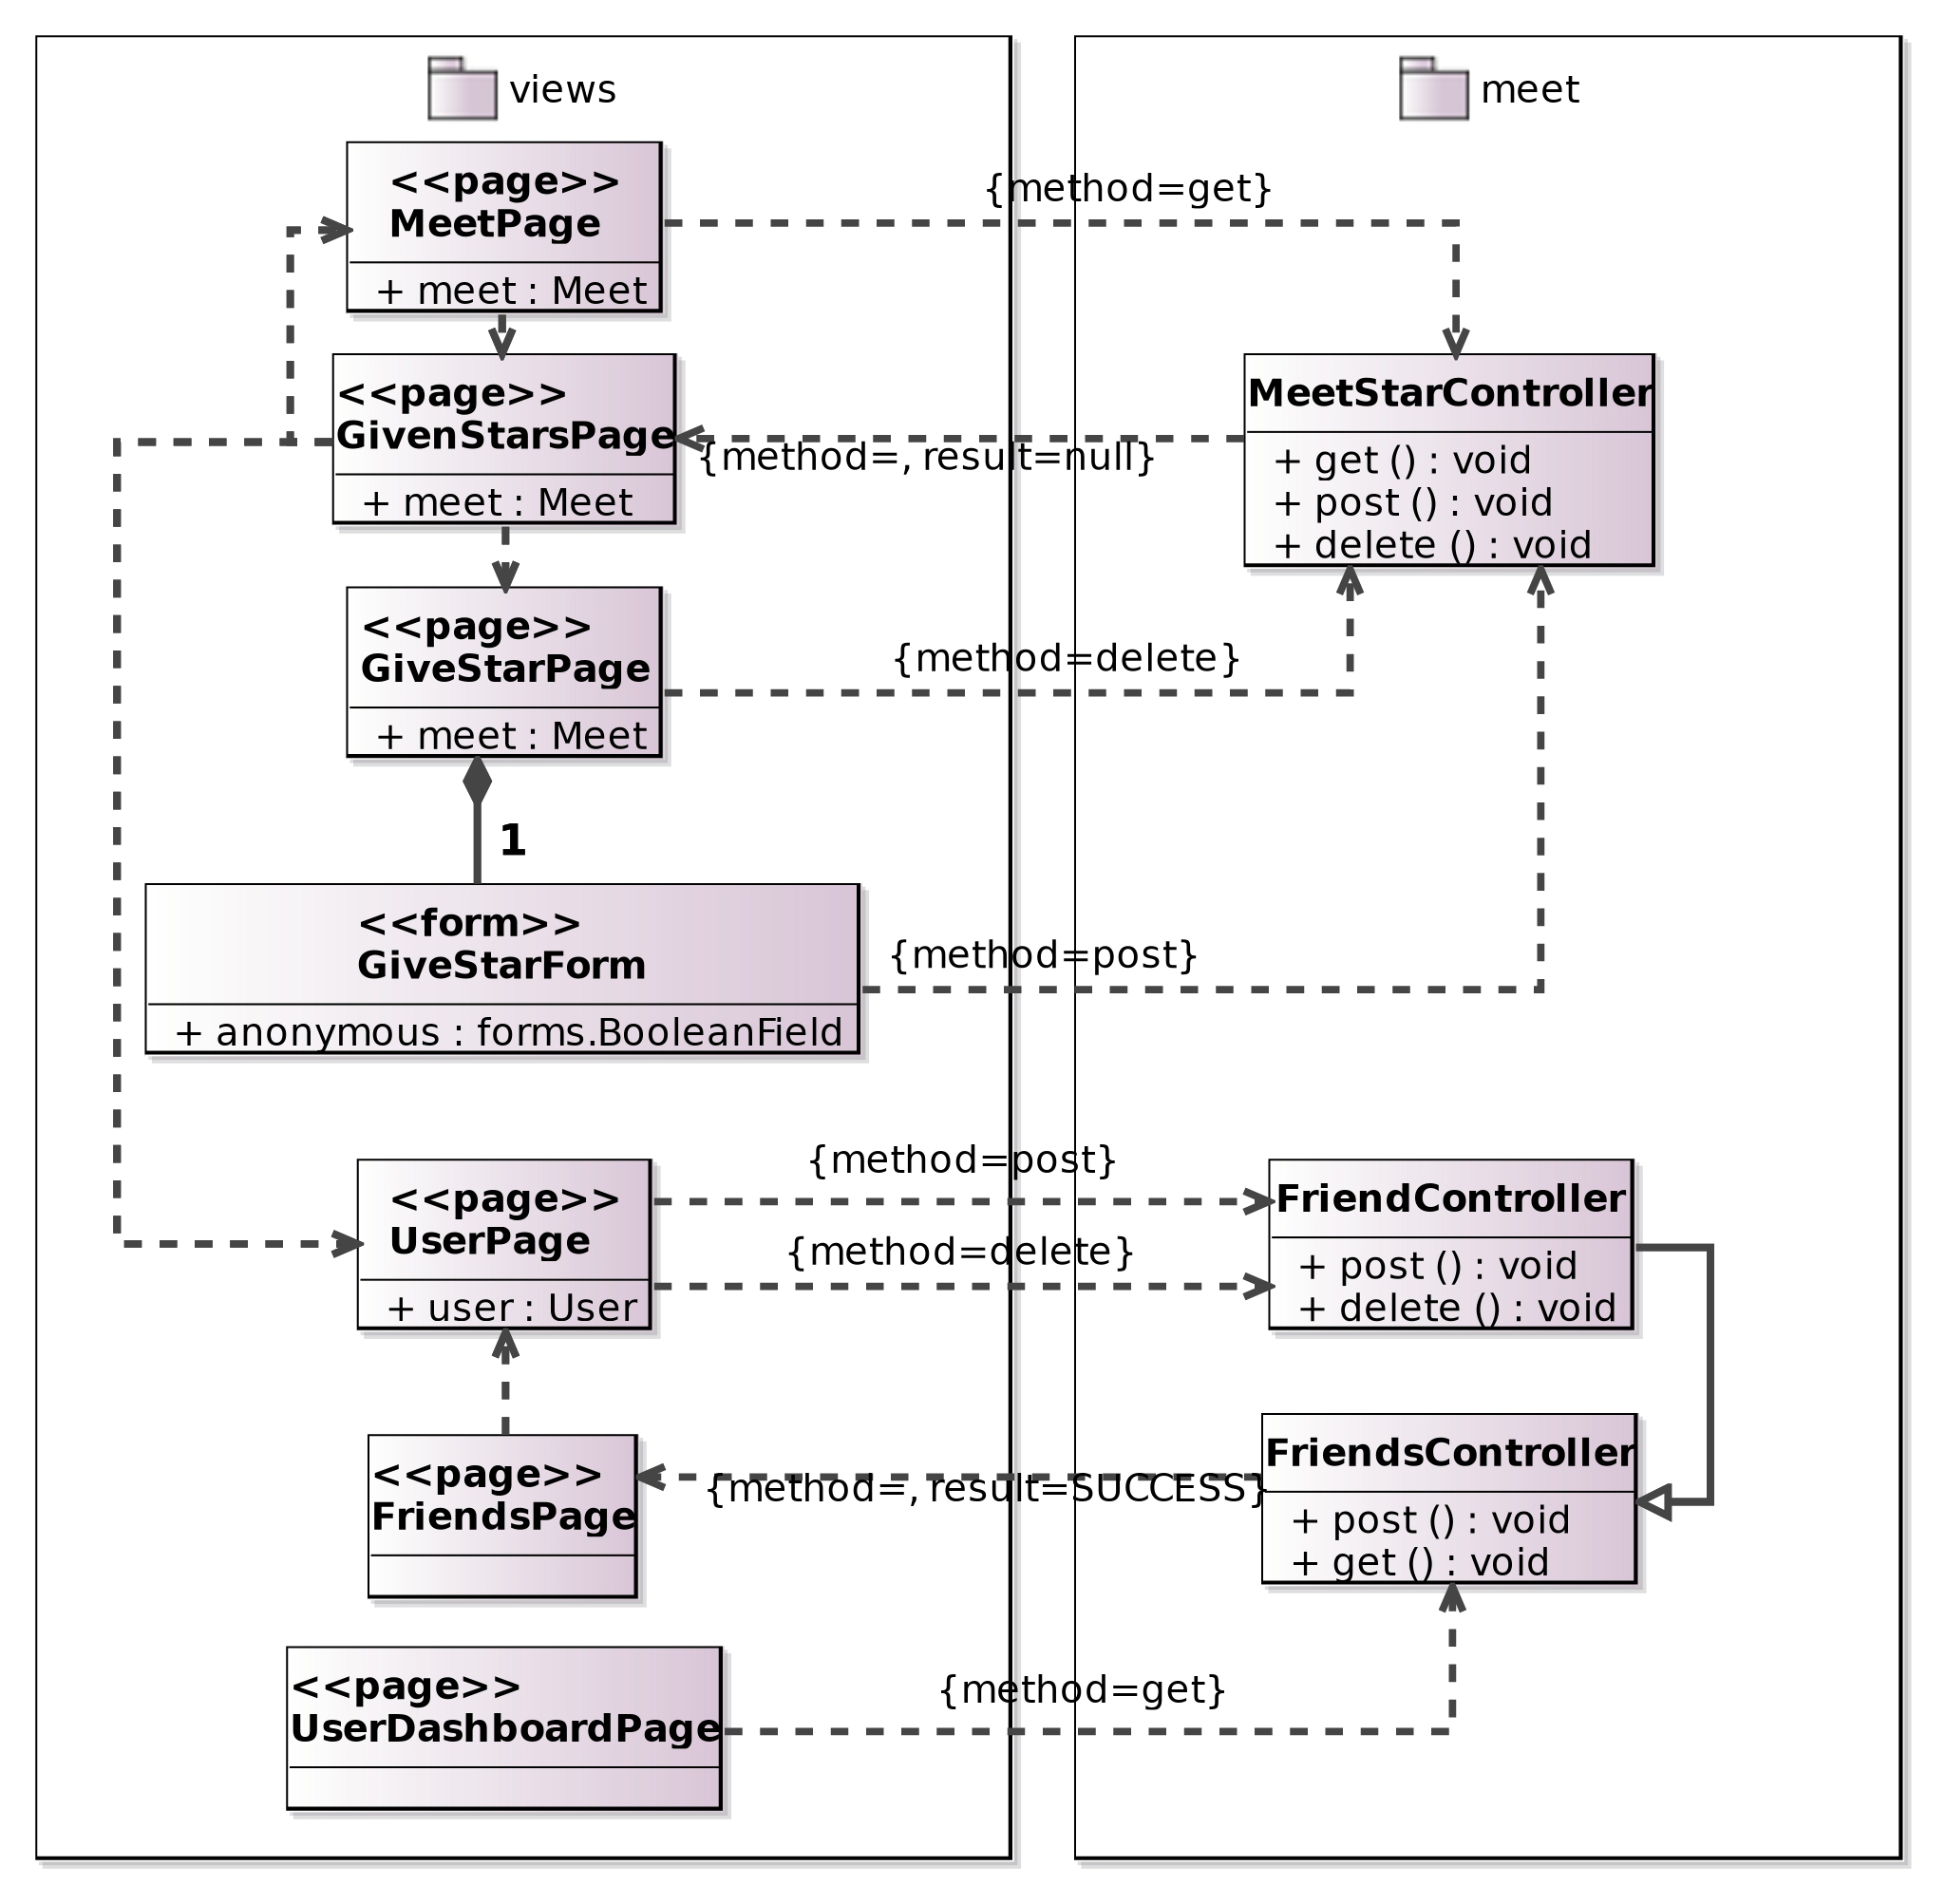
\includegraphics[scale=0.15]{figuras/FrameWebNavigationModel5.jpg}
% 	\caption{Modelo de Navegação do \imprimirtitulo{} -- Participar de encontros e adicionar/aceitar/rejeitar/desistir pedidos de amizade}
% 	\label{fig:nav5}
% \end{figure}
%
% \begin{figure}[H]
% 	\centering
% 	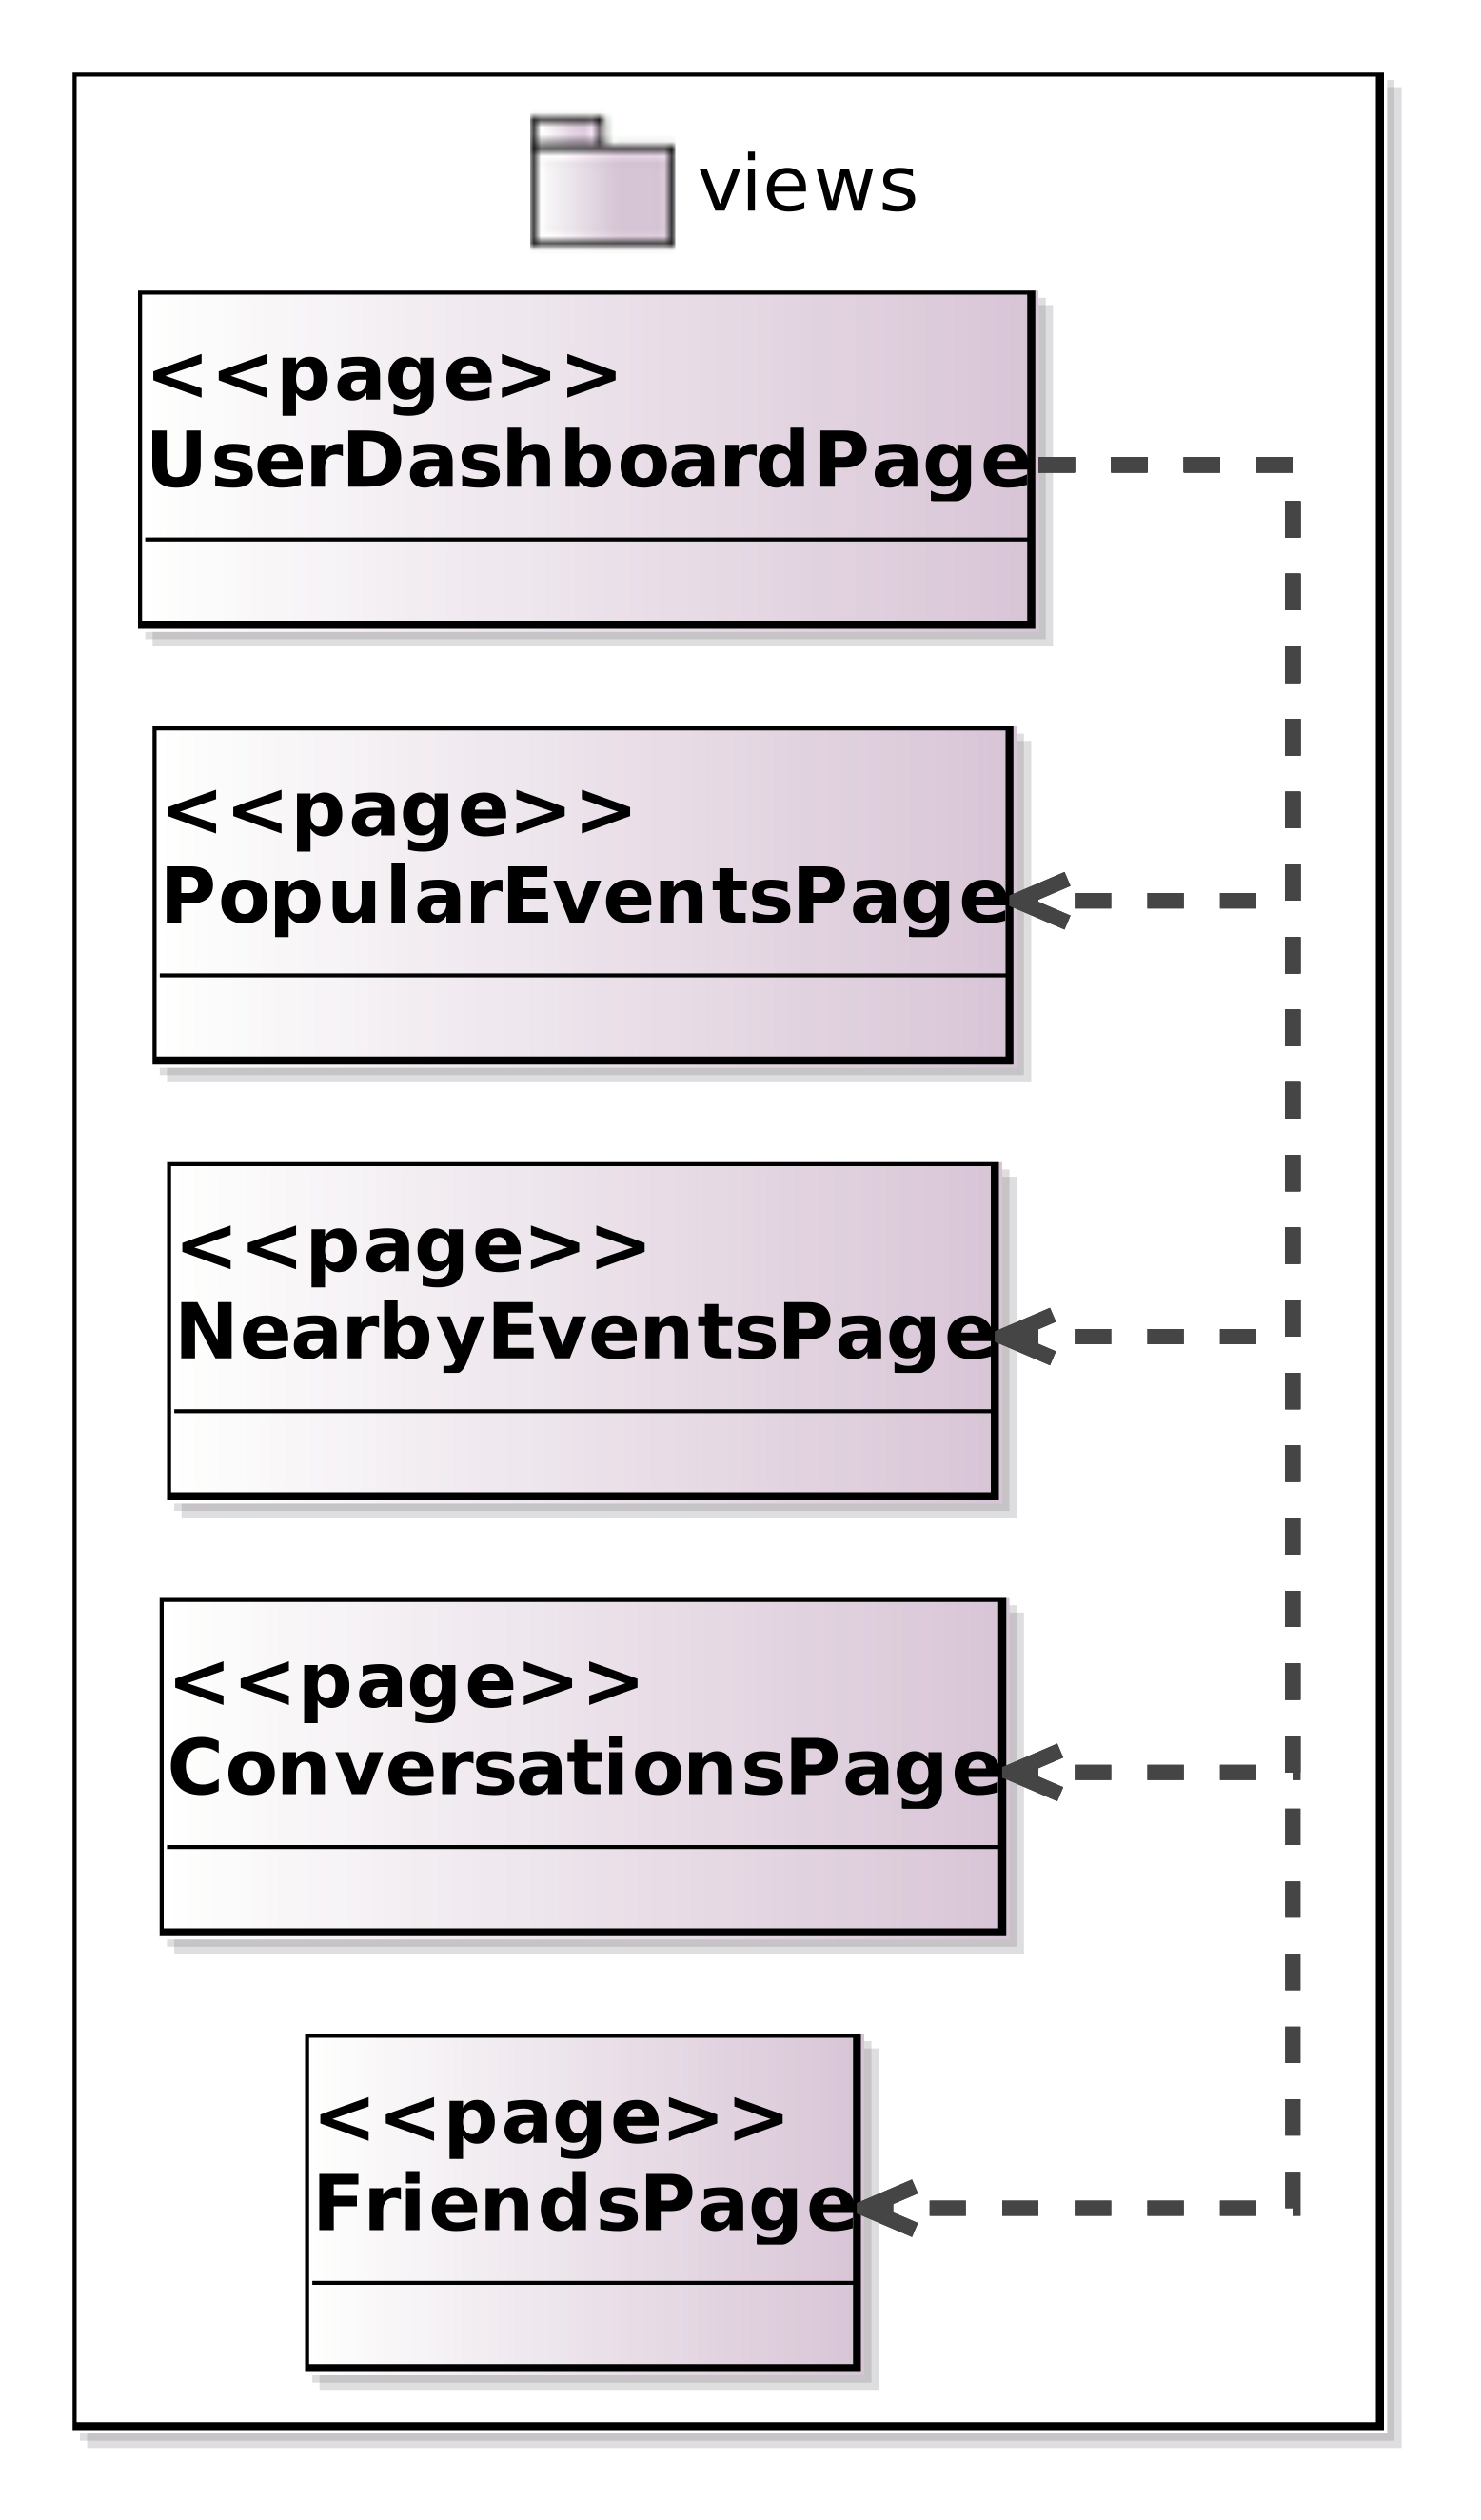
\includegraphics[scale=0.1]{figuras/FrameWebNavigationModel6.jpg}
% 	\caption{Modelo de Navegação do \imprimirtitulo{} -- O caminho do usuário de sua homepage até um ponto em comum com as funcionalidades mencionadas anteriormente; eventuais controladores foram omitidos}
% 	\label{fig:nav6}
% \end{figure}

Embora tal modelo demonstre o sistema como um todo, alguns detalhes podem se perder no meio de tanta abstração, logo, além da funcionalidade de login descrita na Figura \ref{fig:nav1}, a Figura \ref{fig:nav7} e a Figura \ref{fig:nav8} trazem o recorte (sem atalhos) de, respectivamente, enviar uma mensagem para um amigo e de gerenciar os links externos de um encontro.

\begin{figure}[H]
	\centering
	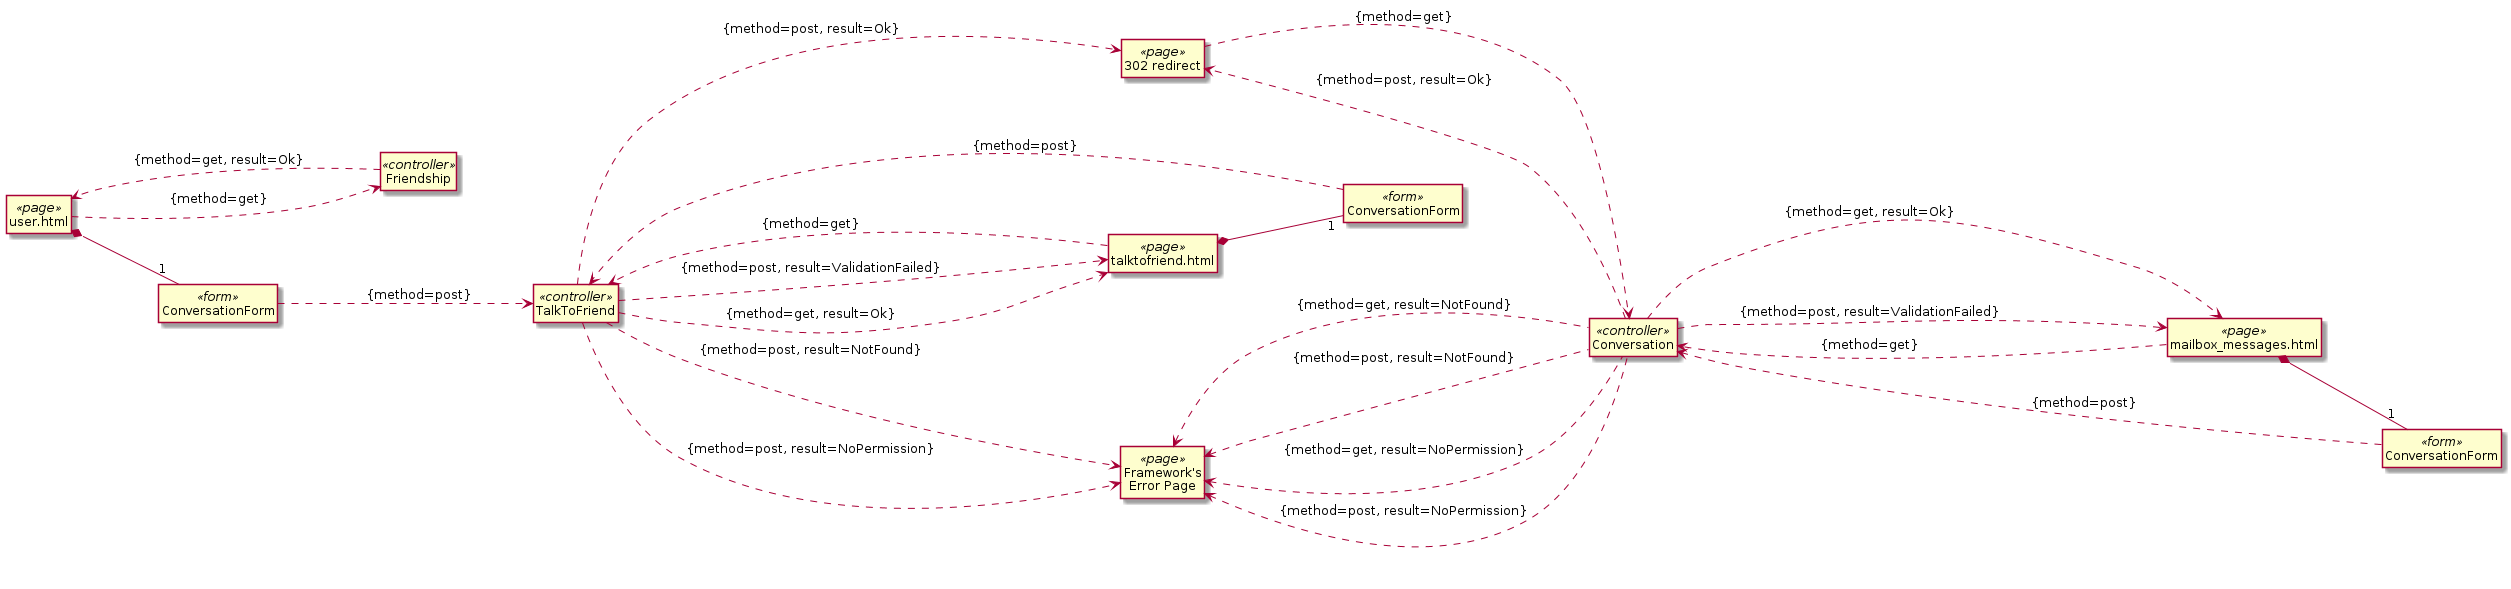
\includegraphics[scale=0.175]{figuras/navspecial1.png}
	\caption{Modelo de Navegação do \imprimirtitulo{} -- Enviar uma mensagem para um amigo}
	\label{fig:nav7}
\end{figure}

\begin{figure}[H]
	\centering
	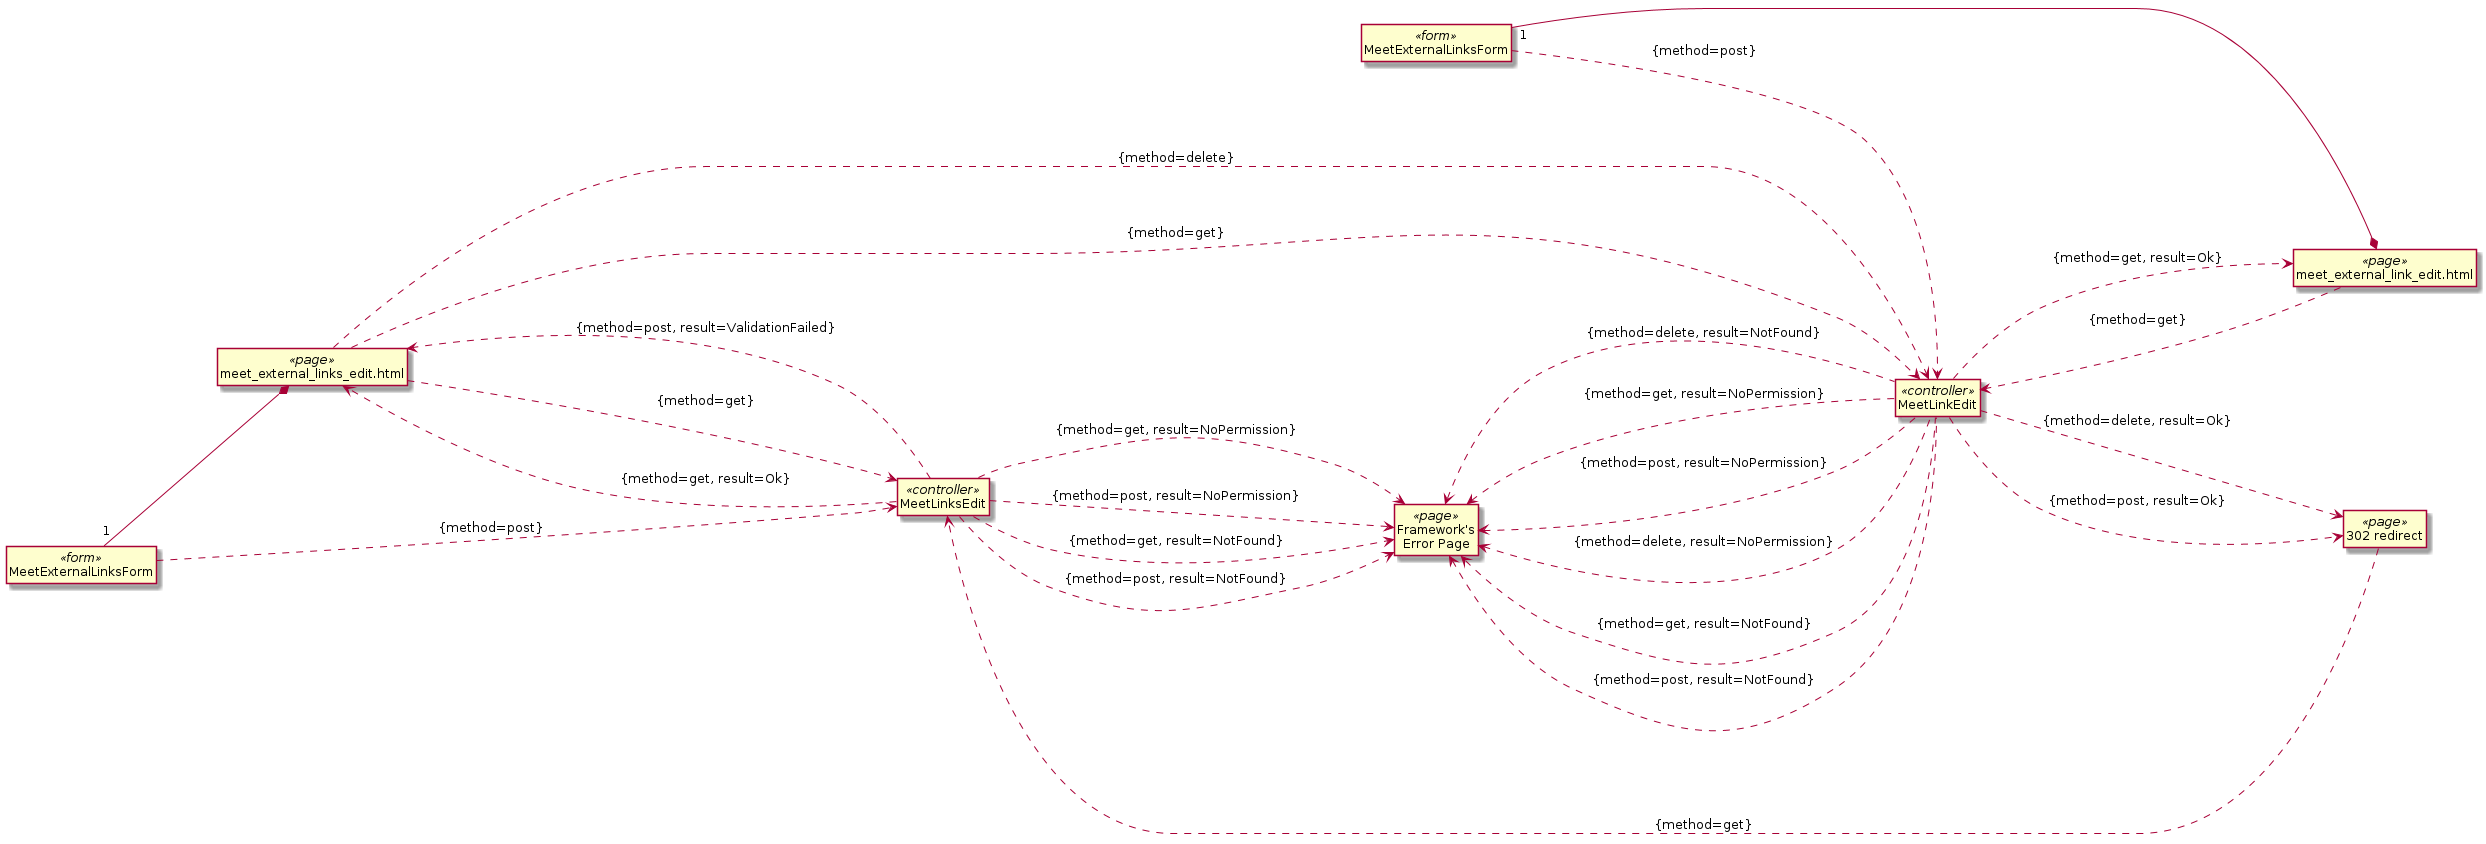
\includegraphics[scale=0.175]{figuras/navspecial2.png}
	\caption{Modelo de Navegação do \imprimirtitulo{} -- Gerenciar os links externos de um encontro}
	\label{fig:nav8}
\end{figure}


\section{Camada de Negócio}
\label{sec-arquitetura-negocio}

% \vitor{Apresentar os modelos de entidades e de aplicação do FrameWeb.}

O modelo de entidades do sistema é composto por uma entidade de usuário (\texttt{User}) que é implementado pela \textit{framework} e uma coleção de entidades próprias, como expresso no pacote \texttt{meet}, que pode ser observado na Figura \ref{fig:ent}.

\begin{figure}[H]
	\centering
	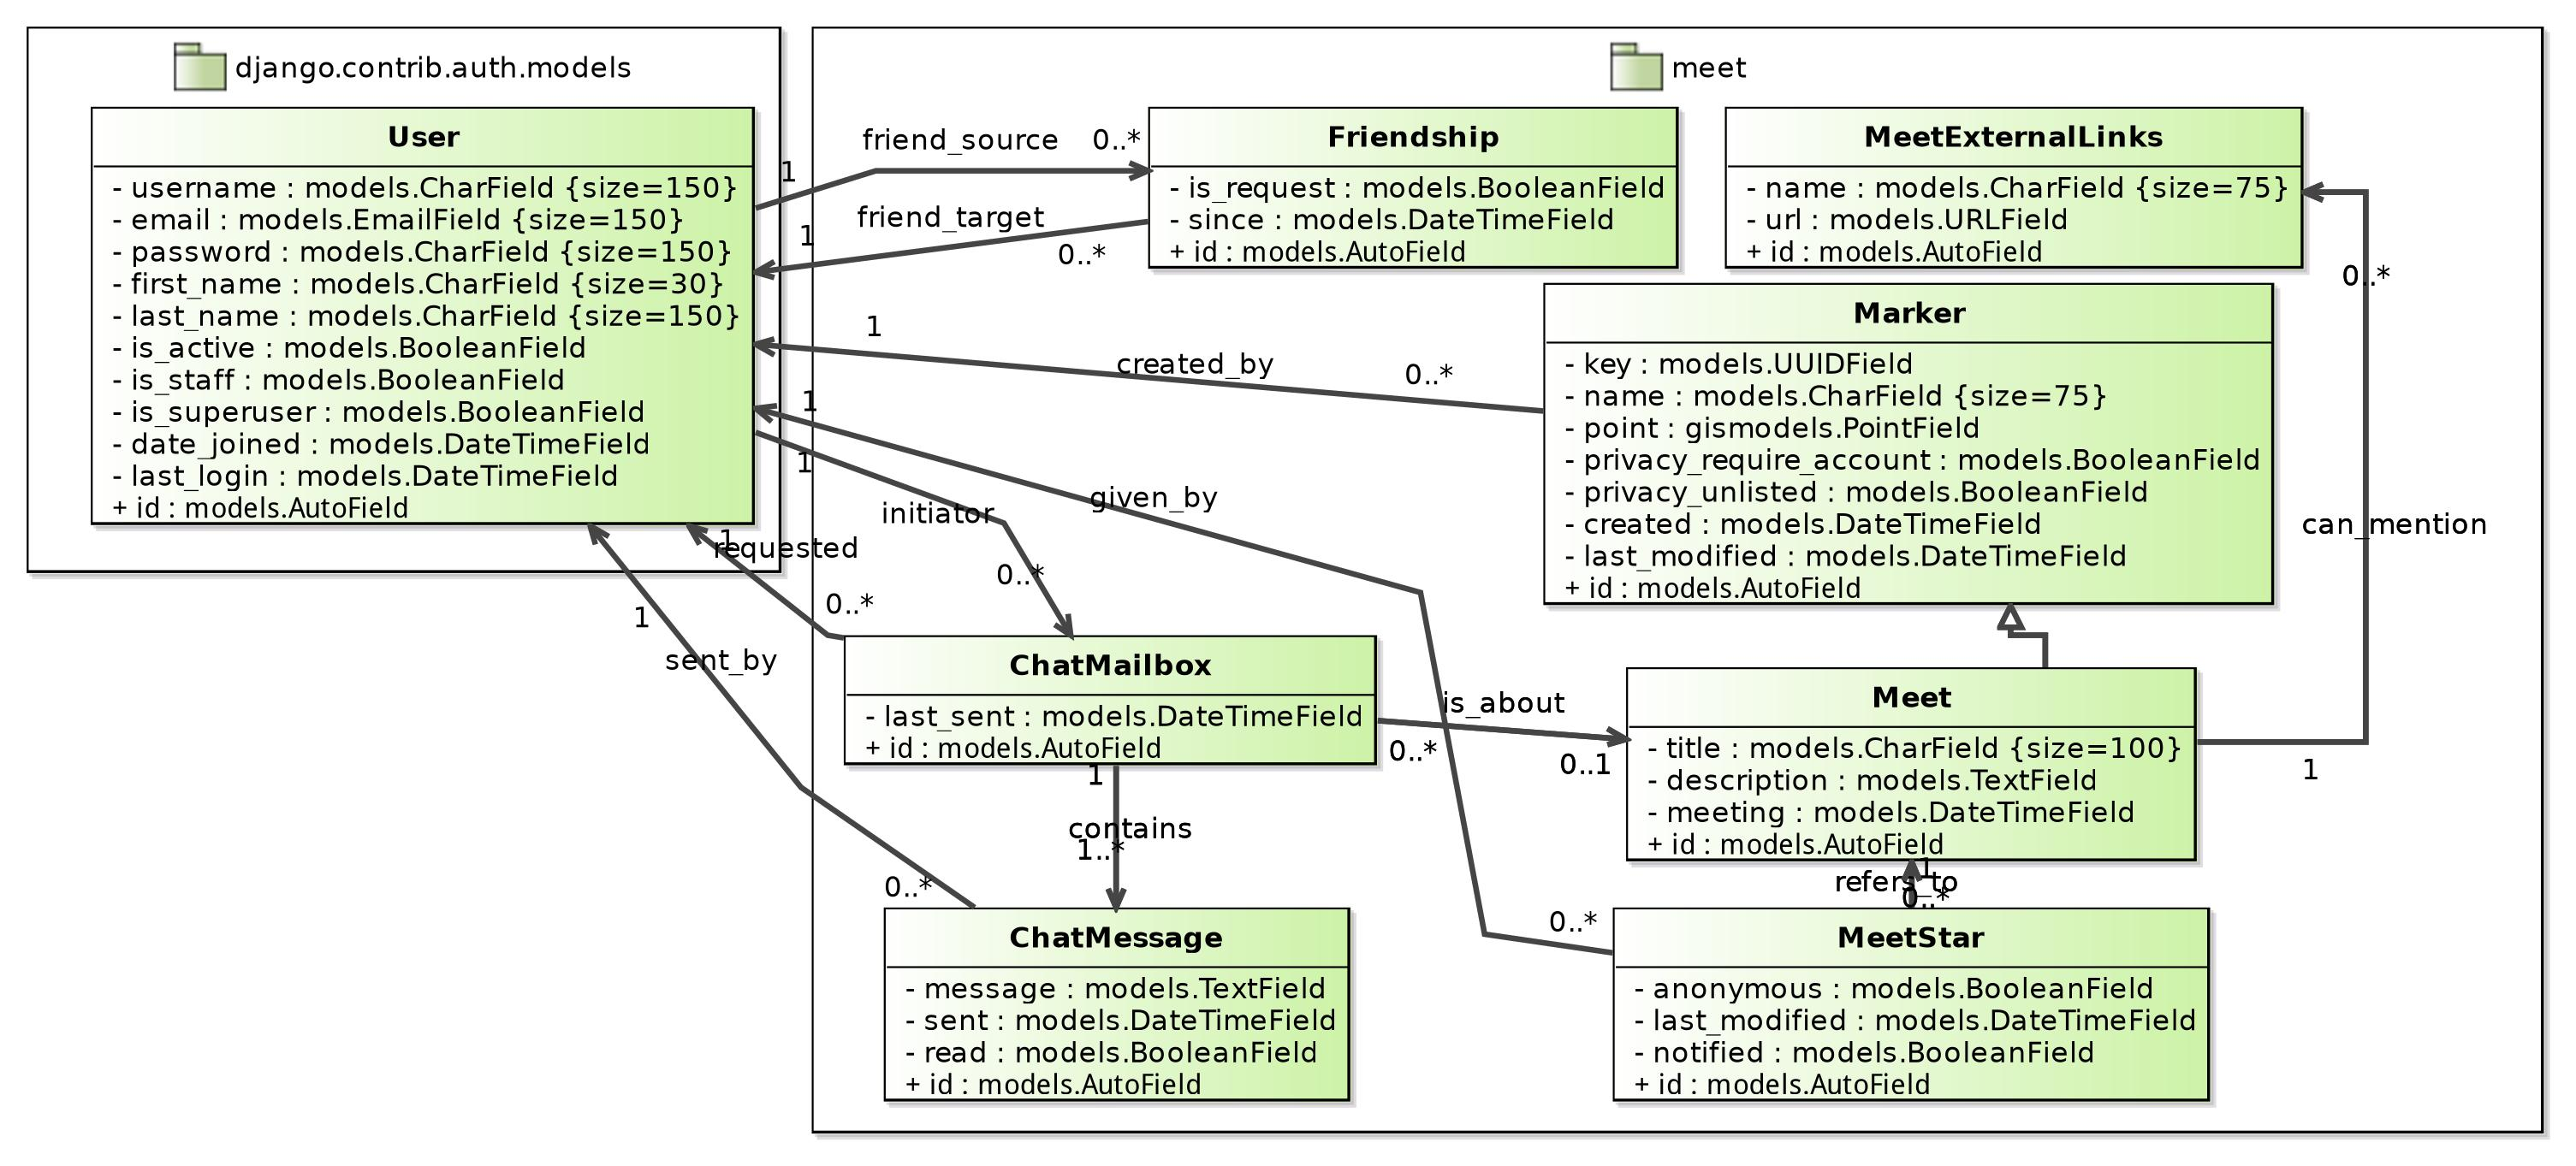
\includegraphics[width=0.8\textwidth]{figuras/FrameWebEntityModel.jpg}
	\caption{Modelo de Entidades do \imprimirtitulo.}
	\label{fig:ent}
\end{figure}

A Figura \ref{fig:ent} possui algumas particularidades devem ser obeservadas:
\begin{itemize}
  \item Todas as classes de modelo herdam de ``\texttt{django.db.models.Model}'', o qual fornece o atrabuto ``\texttt{id}'' (colocado explicitamente em todas as classes neste modelo) como chave primária caso nenhuma outra chave primária seja definida, o que é o caso de todas as classes deste modelo; tal superclasse comum também provê mecanismos relativos à persistência, bem como mecanismos de criação, atualização e busca de elementos, abstraindo completamente detalhes relativos à tecnologia de persistência adotada.
  \item O estereótipo de precisão de datas foi omitido, já que ``\texttt{models.DateTimeField}'' pressupõe implicitamente ``\texttt{\{precision=timestamp\}}'', ``\texttt{models.DateField}'' pressupõe implicitamente ``\texttt{\{precision=date\}}'' e ``\texttt{models.TimeField}'' pressupõe implicitamente ``\texttt{\{precision=time\}}'' e a inclusão deste apenas dificultaria a visualização do modelo.
  \item Todas as associações entre entidades possuem navegabilidade bidirecional, na qual a seta apenas indica o sentido de leitura do rótulo da associação.
  \item Todos os atributos das classes do pacote ``\texttt{meet}'' exceto aqueles decorrentes de associações não podem ser nulos.
  \item Todas as associações exceto ``\texttt{is\_about}'' são representadas por atributos de tipo ``\texttt{models.ForeignKey}'' que não admitem que este armazene nulo.
  \item A associação ``\texttt{is\_about}'' é representada por um atributo de tipo ``\texttt{models.ForeignKey}'' como as outras, mas admitindo valores nulos (devido \`{a} cardinalidade \texttt{0..1}).
  \item Uma instância de \texttt{User} conhece as instâncias de \texttt{Meet} através do atributo de tipo \texttt{models.ForeignKey} herdado de \texttt{Marker}.
  \item Uma instância de \texttt{ChatMailbox} pode simbolizar tanto uma conversa privada entre amigos (ou ex-amigos) quanto uma conversa entre um usuário e o organizador de um encontro sobre o encontro: se a associação ``\texttt{is\_about}'' do lado \texttt{ChatMailbox} possuir um \texttt{Meet}, é uma conversa entre um usuário e o organizador de um encontro sobre o encontro; caso contrário, é uma conversa privada.
  \item Uma instância de \texttt{ChatMailbox} possui 2 atributos de tipo ``\texttt{models.ForeignKey}'' derivados de associações entre esta entidade e \texttt{User} (explicitamente, as associações ``initiator'' e ``requsted'') que armazenam na classe ``\texttt{ChatMailbox}'' quem começou a conversa e quem receberia a primeira mensagem da conversa.
  \item A classe \texttt{Meet} e \texttt{Marker} estão separadas em classes diferentes para facilitar estender, futuramente, funcionalidades no sistema.
  \item A classe \texttt{User} é fornecida ou pelo \textit{framework}; está presente no modelo apenas para favorecer a completude .
\end{itemize}

A camada de aplicação do modelo é expressa pela Figura \ref{fig:apl}, a qual é redundante com a assinatura dos métodos dos controladores apresentados na Figura \ref{fig:nav0}, mas de uma forma diferente com menos texto.

\begin{figure}[H]
	\centering
	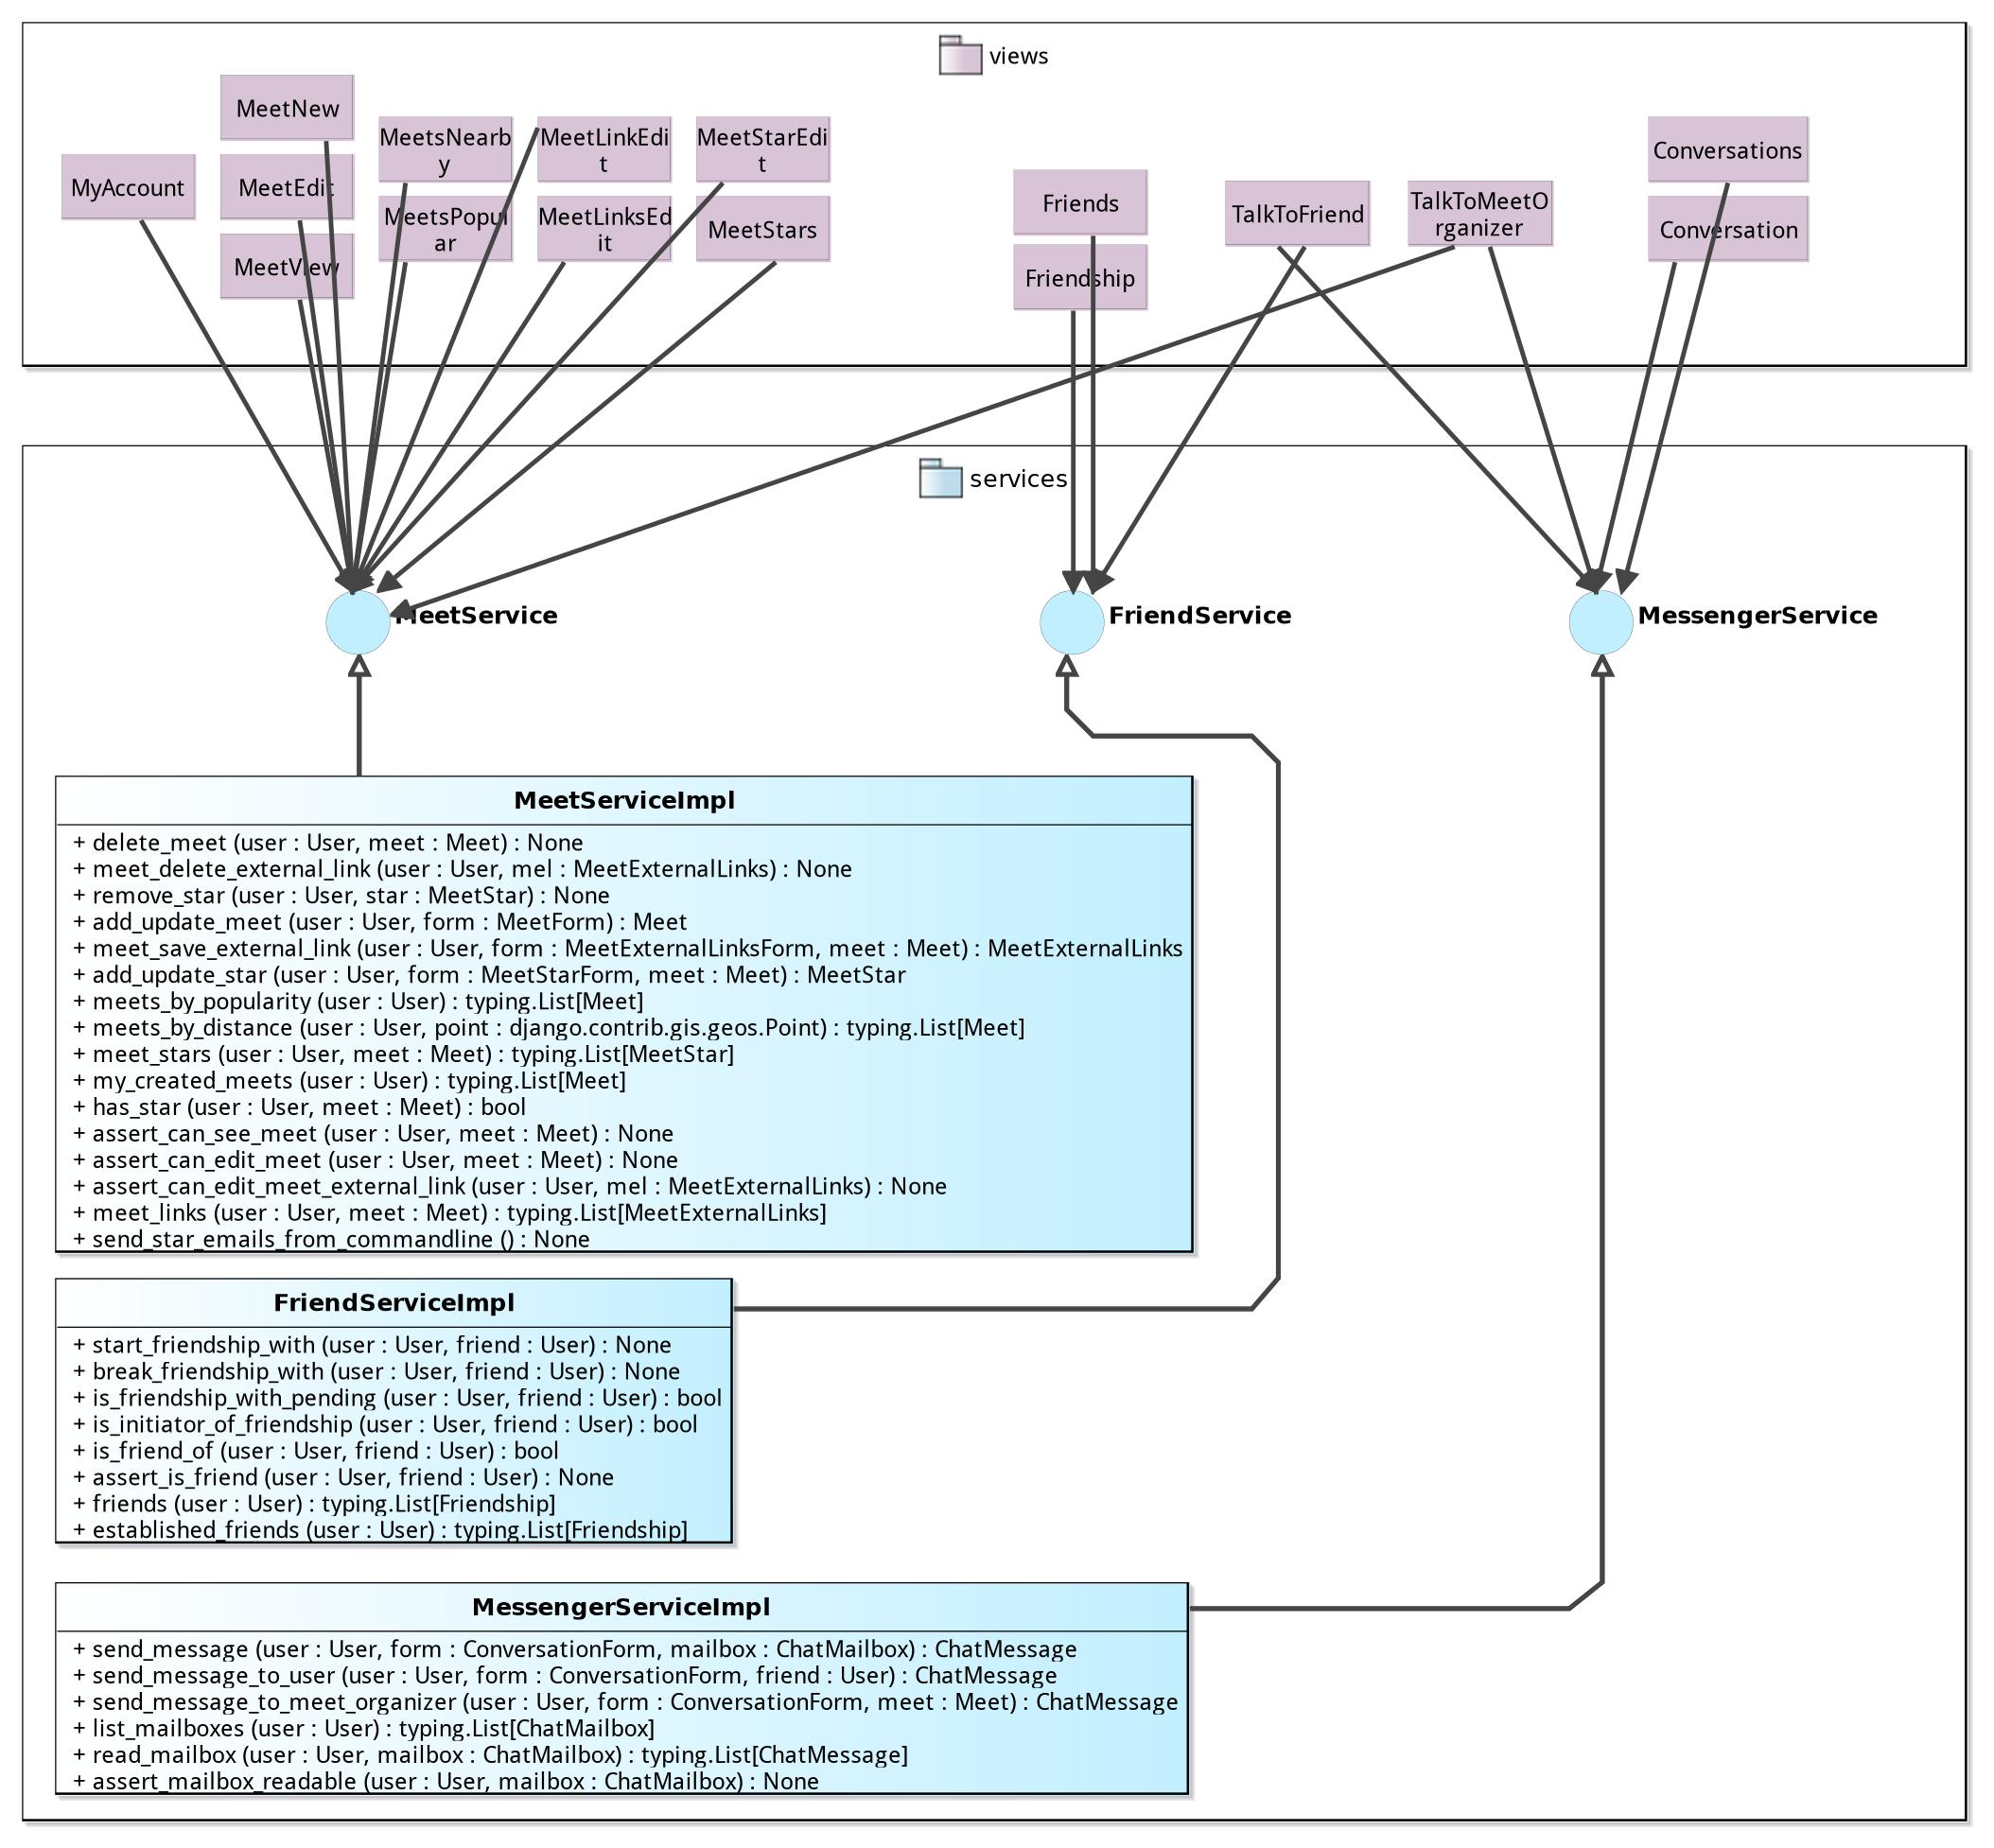
\includegraphics[width=0.8\textwidth]{figuras/FrameWebApplicationModel.jpg}
	\caption{Modelo de Aplicação do \imprimirtitulo.}
	\label{fig:apl}
\end{figure}

Como Django usa \textit{Active Record} e não \textit{Data Access Objects} e, por conta disso, a camada de acesso ao dado foi ignorada, e, por conseguinte, o modelo de persistência não existir, a Figura \ref{fig:ese} explicita quais modelos são gerenciados por quais serviços, suprindo a lacuna causada pela falta deste. Apesar do serviço \texttt{LDService} não gerenciar nenhuma entidade, ele expõe as entidades a ele relacionadas, conforme será apresentado na seção \ref{mfld}.

\begin{figure}[H]
	\centering
	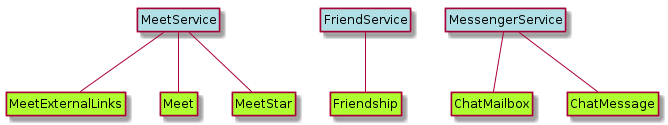
\includegraphics[width=0.8\textwidth]{figuras/entidade-servico-escrita.png}
	\caption{Modelo que explicita a relação de gerência das entidades pelos serviços do sistema.}
	\label{fig:ese}
\end{figure}

\subsection{Modelo Frameweb-LD}
\label{mfld}

\begin{figure}[H]
	\centering
	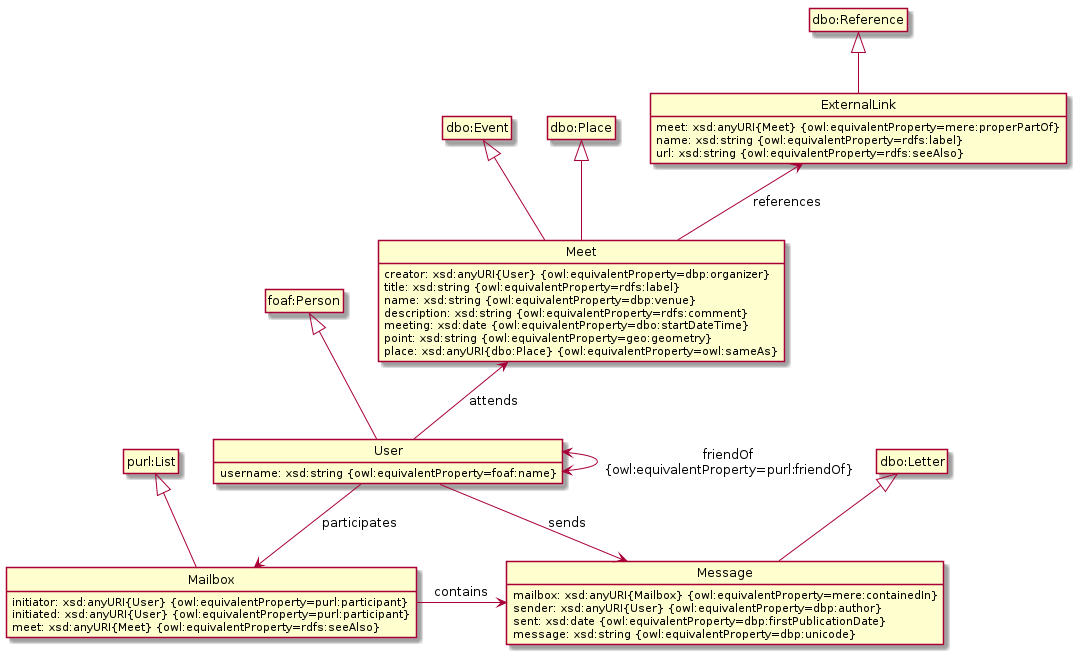
\includegraphics[width=0.8\textwidth]{figuras/framewebld.png}
	\caption{Modelo de Entidades de \textit{Linked Data} do \imprimirtitulo.}
	\label{fig:ld}
\end{figure}

A Figura \ref{fig:ld} mostra a versão \textit{Linked Data} exposta das entidades da Figura \ref{fig:ent}.
A classe \texttt{ChatMailbox} foi exposta como \texttt{Mailbox}.
A classe \texttt{ChatMessage} foi exposta como \texttt{Message}.
A classe \texttt{MeetExternalLinks} foi exposta como \texttt{ExternalLink}.
A classe \texttt{Friendship} foi exposta apenas como uma relação entre duas entidades.
A propriedade \texttt{place} da classe \texttt{Meet} da Figura \ref{fig:ld} é dada pela propriedade \texttt{point\_ld} da classe de mesmo nome na Figura \ref{fig:ent}.
A propriedade \texttt{meet} da classe \texttt{ExternalLink} da Figura \ref{fig:ld} é dada pela propriedade \texttt{parent} da classe equivalente na Figura \ref{fig:ent}.
De resto, o modelo continua representando os mesmos dados, ainda que usando nomes ligeiramente diferentes e explicitando a presença de algumas propriedades cuja presença era apenas presumida a partir das associações presentes na Figura \ref{fig:ent} e mantendo outras ainda presumidas.

% \section{Camada de Acesso a Dados}
% \label{sec-arquitetura-dados}
%
% \vitor{Apresentar os modelos de persistência do FrameWeb.}
